\documentclass[12pt,oneside,letterpaper,chapterprefix=on,numbers=noenddot]{scrbook}

\usepackage{todonotes}
\usepackage{dirtytalk}
\usepackage[normalem]{ulem}   % underline for section headings per CSULB format

% CSULB thesis margins: 1.5" left, 1" right/top/bottom.
% First page of each chapter gets an extra 1" of vertical space before the
% chapter title, producing the required 2" top on chapter opening pages.
\usepackage[left=1.5in,right=1in,top=1in,bottom=1in,includefoot,heightrounded]{geometry}
\usepackage[T1]{fontenc}   % required for non-English accents (e.g. the ogonek in "Gąsieniec")
\usepackage{mathptmx}
\usepackage{setspace}
\usepackage{indentfirst}
\setlength{\parindent}{0.5in}
\usepackage[document]{ragged2e}
\setlength{\RaggedRightParindent}{\parindent}
\usepackage{comment}
\pagestyle{plain}
\usepackage[justification=raggedright,singlelinecheck=false,labelsep=period]{caption}
\setkomafont{captionlabel}{\bfseries}
\setkomafont{caption}{\bfseries}
\setcapindent{0pt}
\usepackage{graphicx}
\graphicspath{{../figures/}{figures/}}
\usepackage{amsmath,amssymb,amsthm}
\usepackage{enumitem}
\usepackage{booktabs}

\tolerance=1
\emergencystretch=\maxdimen
\hyphenpenalty=10000
\hbadness=10000

\usepackage{algorithm}
\makeatletter
\renewcommand{\ALG@name}{ALGORITHM}
\captionsetup[algorithm]{labelfont=bf,labelsep=period,font=bf}
\makeatother
\usepackage{algpseudocode}
\algdef{SE}[DOWHILE]{Do}{DoWhile}{\algorithmicdo}[1]{\algorithmicwhile\ #1}

\newtheoremstyle{csulb}
  {\topsep}{\topsep}{\normalfont}{0.25in}{\itshape}{{\normalfont :\ } }{0pt}
  {\thmname{#1} \thmnumber{#2}}
\theoremstyle{csulb}
\newtheorem{theorem}{Theorem}
\newtheorem{lemma}{Lemma}
\newtheorem{corollary}{Corollary}
\newtheorem{definition}{Definition}
\newtheorem{problem}{Problem}

\DeclareOldFontCommand{\bf}{\normalfont\bfseries}{\mathbf}
\newcommand{\argmax}{\operatornamewithlimits{argmax}}

% APA-style author-year inline citations per CSULB Honors requirements.
% round  = parentheses around citations
% authoryear = "(Author, Year)" format instead of numeric [1]
% sort&compress = alphabetical order, compressed ranges
\usepackage[round,authoryear,sort&compress]{natbib}
\setlength{\bibsep}{0pt}
\setcounter{secnumdepth}{0}

% Renames the "Bibliography" section heading to "REFERENCES" (CSULB spec).
\renewcommand{\bibname}{REFERENCES}

\makeatletter
\renewcommand\chapterlinesformat[3]{\@hangfrom{#2}{\MakeUppercase{#3}}}
\makeatother
\renewcommand\chapterlineswithprefixformat[3]{\MakeUppercase{#2#3}}

\usepackage{chngcntr}
\counterwithout{figure}{chapter}
\counterwithout{table}{chapter}

\let\raggedchapter\centering
% 1in beforeskip + 1in top page margin = 2" to chapter title (CSULB rule).
% 0.25in afterskip between chapter title and first paragraph.
\RedeclareSectionCommand[beforeskip=1in,afterskip=0.25in]{chapter}
\setkomafont{disposition}{\bfseries\normalsize}
\setkomafont{chapter}{\normalsize}
\let\raggedsection\centering
\setkomafont{section}{\normalsize}
\RedeclareSectionCommand[beforeskip=0pt,afterskip=0.01pt]{section}
\setkomafont{subsection}{\normalsize}
\RedeclareSectionCommand[beforeskip=0pt,afterskip=0.01pt]{subsection}

% CSULB format: first/second-level subheads centered/left + underlined.
\makeatletter
\renewcommand\sectionlinesformat[4]{%
  \@hangfrom{\hskip #2#3}{\uline{#4}}%
}
\makeatother

% CSULB format: third-level run-in subheads are underlined, NOT bold.
% All \paragraph{} uses in this thesis have no optional argument,
% so a simple two-argument patch is safe.
\setkomafont{paragraph}{\normalsize\mdseries}
\makeatletter
\let\csulb@oldparagraph\paragraph
\renewcommand\paragraph[1]{\csulb@oldparagraph{\uline{#1}}}
\makeatother

\usepackage{etoolbox}
\AtBeginEnvironment{figure}{\setlength{\RaggedRightParindent}{0em}}
\AtBeginEnvironment{table}{\setlength{\RaggedRightParindent}{0em}}
\AtBeginEnvironment{algorithm}{\setlength{\RaggedRightParindent}{0em}}

\usepackage{tocloft}
\setlength{\cftbeforetoctitleskip}{0pt}
\setlength{\cftaftertoctitleskip}{0pt}
\renewcommand*\contentsname{TABLE OF CONTENTS}
\renewcommand{\cfttoctitlefont}{\hspace*{\fill}\normalsize}
\renewcommand{\cftaftertoctitle}{\hspace*{\fill}}
\KOMAoptions{toc=chapterentrydotfill}
\setkomafont{chapterentry}{}
\addtokomafont{chapterentrypagenumber}{\mdseries}
\RedeclareSectionCommand[tocnumwidth=3.5em]{chapter}

\setlength{\cftbeforelottitleskip}{0pt}
\setlength{\cftafterlottitleskip}{0pt}
\renewcommand*\listtablename{LIST OF TABLES}
\renewcommand{\cftlottitlefont}{\hspace*{\fill}\normalsize}
\renewcommand{\cftafterlottitle}{\hspace*{\fill}}
\setlength{\cfttabindent}{0.25in}

\setlength{\cftbeforeloftitleskip}{0pt}
\setlength{\cftafterloftitleskip}{0pt}
\renewcommand*\listfigurename{LIST OF FIGURES}
\renewcommand{\cftloftitlefont}{\hspace*{\fill}\normalsize}
\renewcommand{\cftafterloftitle}{\hspace*{\fill}}
\setlength{\cftfigindent}{0.25in}
\newcommand*{\noaddvspace}{\renewcommand*{\addvspace}[1]{}}
\addtocontents{lof}{\protect\noaddvspace}
\addtocontents{lot}{\protect\noaddvspace}

\renewenvironment{proof}{\indent{\em Proof}:}{}

\usepackage[page,toc,title]{appendix}
\renewcommand{\appendixtocname}{APPENDIX}
\renewcommand{\appendixpagename}{\vspace*{\fill}\centering\normalsize APPENDIX\vspace*{\fill}}

\usepackage{hyperref}
\hypersetup{colorlinks,citecolor=black,linkcolor=black,urlcolor=black}

\usepackage[english]{babel}
\addto\captionsenglish{\renewcommand{\contentsname}{TABLE OF CONTENTS}}
\addto\captionsenglish{\renewcommand{\listfigurename}{LIST OF FIGURES}}
\addto\captionsenglish{\renewcommand{\listtablename}{LIST OF TABLES}}
\captionsetup{figurename=FIGURE,tablename=TABLE}

\begin{document}

\frontmatter
% Front matter uses lowercase Roman numerals (scrbook default under
% \frontmatter). Title page is counted as page i but prints no number
% per CSULB rules; \mainmatter restarts Arabic numbering at 1 below.

\pagenumbering{roman}
% CSULB rule: title page counts as page i but displays no number.
% Template requires ALL text on the title page to be bold.
\pagestyle{empty}
\thispagestyle{empty}
\begin{doublespacing}
\begin{center}
\bfseries
\vspace*{0.5in}
ON THE NUMERICAL ANALYSIS OF MULTI-ROBOT SEARCH\\
AND RESCUE ALGORITHMS IN UNKNOWN\\
ENVIRONMENTS

\vspace{0.75in}
A THESIS

\vspace{0.5in}
Presented to the University Honors Program

California State University, Long Beach

\vspace{0.5in}
In Partial Fulfillment\\
of the Requirements for the\\
University Honors Program Certificate

\vspace{0.75in}
Fozhan Babaeiyan Ghamsari

\vspace{0.5in}
Spring 2026
\end{center}
\end{doublespacing}
\clearpage

\thispagestyle{empty}
% Restore plain page style after signature page so Roman numbering
% appears starting at the abstract.
\begin{doublespacing}
\begin{center}
\vspace*{0.5in}
I, THE UNDERSIGNED MEMBER OF THE COMMITTEE,\\
HAVE APPROVED THIS THESIS

\vspace{0.5in}
\textbf{ON THE NUMERICAL ANALYSIS OF MULTI-ROBOT SEARCH\\
AND RESCUE ALGORITHMS IN UNKNOWN\\
ENVIRONMENTS}

\vspace{0.5in}
BY

\vspace{0.25in}
Fozhan Babaeiyan Ghamsari

\vspace{0.75in}
\begin{tabular}{p{3.5in}p{1.5in}}
\hrulefill & \\
Oscar Morales-Ponce, Ph.D. (Thesis Advisor) & Computer Engineering and Computer Science \\
\end{tabular}

\vspace{0.75in}
California State University, Long Beach

\vspace{0.25in}
Spring 2026
\end{center}
\end{doublespacing}
\pagestyle{plain}
\clearpage


\clearpage
\phantomsection
\addcontentsline{toc}{chapter}{ABSTRACT}
\begin{center}
ABSTRACT

\vspace{0.25in}
ON THE NUMERICAL ANALYSIS OF MULTI-ROBOT SEARCH\\
AND RESCUE ALGORITHMS IN UNKNOWN\\
ENVIRONMENTS

\vspace{0.25in}
By

\vspace{0.1in}
Fozhan Babaeiyan Ghamsari

\vspace{0.1in}
Spring 2026
\end{center}

\begin{doublespacing}
\noindent
Every minute after a structural collapse, the probability of finding
survivors alive decreases. When autonomous robot teams are deployed to
search collapsed buildings, earthquake rubble, or flood sites, they
face two simultaneous constraints: a finite battery budget that forces
frequent returns to a charging base, and limited inter-robot
communication that makes coordination difficult.
This thesis studies the multi-robot search and rescue problem in which
$R$ robots must locate a target hidden among $n$ candidate sites, each
carrying a prior probability $p_i$ of containing the target, under a
finite per-robot energy budget $E$. Four algorithmic models spanning
the energy--communication design space are introduced and compared:
M1, an uncoordinated random baseline with \emph{no inter-robot
communication whatsoever}; M2, which introduces
\emph{Sequential Single-Item (SSI) auctions} with unconstrained energy;
M3, which adds the energy constraint with a standard $p_i/d$ bid
function; and M4/M4*, which extends each sortie via a \emph{greedy
chain extension} using the novel $p_i/d^2$ bid, alongside a
\emph{Hungarian assignment} baseline for comparison.
Performance is measured by the \emph{Finder Competitive Ratio} (FCR),
the ratio of the finding robot's travel distance to the omniscient
optimum, for which closed-form upper bounds are derived for each model.
All bounds are validated through 5,000 Monte Carlo trials in a
$10 \times 10$ square arena with $n = 30$ candidate sites and
$R = 3$ robots, with parameter sweeps over the energy budget
$E \in [8, 30]$ and fleet size $R \in [1, 6]$.
Four results emerge from this study.
Auction-based coordination yields a 6.6-fold improvement in FCR over
uncoordinated random search.
SSI auctions with probability-aware bids outperform Hungarian
assignment by $8.1\%$, and adding probability weighting to Hungarian
assignment alone \emph{worsens} performance due to a clustering
pathology, establishing that the SSI iterative bid-update mechanism
is essential.
Multi-node greedy chains recover $90\%$ of the performance gap between
energy-constrained and unconstrained operation.
The novel $p_i/d^2$ bid function outperforms the standard $p_i/d$ bid
by $1.5\%$ overall, with the advantage growing to approximately $12\%$
at tight energy budgets, justified by a cost-foreclosure argument
showing that a distant anchor site not only costs more energy to reach
but also shrinks the budget available for subsequent chain extensions.
Therefore, this thesis provides a reproducible foundational benchmark,
with closed-form guarantees and simple one-line deployment rules,
applicable to any scenario in which a team of resource-constrained
agents must locate a target under uncertainty---from urban
search-and-rescue to autonomous planetary exploration.
\end{doublespacing}
\clearpage

\clearpage
\phantomsection
\addcontentsline{toc}{chapter}{ACKNOWLEDGMENTS}
\begin{center}
\textbf{ACKNOWLEDGMENTS}
\end{center}

\begin{doublespacing}
\noindent
I would like to thank my thesis advisor, Dr.\ Oscar Morales-Ponce, for
his guidance throughout this research, for the many hours of discussion
that sharpened the ideas in this thesis, and for his patience in
helping me translate intuitions into formal arguments. I am grateful
to the Department of Computer Engineering and Computer Science and to
the University Honors Program at California State University, Long
Beach, for providing the structure and the community that made this
work possible. Finally, I thank my family for their steady support
throughout my undergraduate studies.
\end{doublespacing}
\clearpage


\begin{doublespacing}
  \clearpage
  \tableofcontents
  \renewcommand{\autodot}{.}

  \clearpage
  \phantomsection
  \listoftables
  \addcontentsline{toc}{chapter}{LIST OF TABLES}

  \clearpage
  \phantomsection
  \listoffigures
  \addcontentsline{toc}{chapter}{LIST OF FIGURES}
\end{doublespacing}

\mainmatter
\pagenumbering{arabic}      % body pages: Arabic numerals starting at 1
\RaggedRight                 % CSULB rule: no right-justification in body

\chapter{INTRODUCTION}\label{ch:intro}

\begin{doublespacing}

In the minutes and hours after a building collapses, collapsed-structure
entry is dangerous for human rescuers and a high-stakes information
problem: a survivor is somewhere in a rubble field and the probability
that they are in any particular void pocket is unevenly distributed.
Small autonomous robots---aerial drones, crawling ground units, or
tethered probes---can be deployed into the structure to search. When
several robots are available, the question becomes not merely
\emph{where should a robot look} but \emph{how should a team of robots
divide the search}. Poor coordination causes robots to check the same
locations and to burn their finite batteries before checking the most
likely ones. Good coordination \emph{on the right mathematical
foundations} can cut search distance dramatically, and it is those
foundations that this thesis studies.

This thesis addresses the following question. Given a team of $R$
battery-powered robots, a set of $n$ candidate survivor locations with
non-uniform prior probabilities, and a worst-case metric of efficiency,
what combination of communication assumptions, bid functions, and
routing decisions minimizes the distance a robot travels before finding
the target? The answer, which this thesis develops formally and
validates numerically, is that the bottleneck is not fleet size or
battery capacity in isolation but the bid function that robots use to
decide which site to visit next, together with their ability to chain
several sites into a single energy-feasible tour.

\section{Motivation}

Urban search-and-rescue (USAR) robotics has matured from tele-operated
single-unit deployments toward teams of semi-autonomous robots. Field
reports from deployments at the World Trade Center~\cite{Casper2003},
the Fukushima Daiichi plant, and several recent earthquakes consistently
identify two practical pain points: robots exhaust their batteries
before finishing their search, and multiple robots redundantly cover
the same ground when communication links drop. The two problems are
related. Under strict energy budgets, each wasted sortie---that is,
each excursion that checks a site of low prior probability or revisits
a site that a teammate already cleared---is a larger fraction of the
total searchable volume. Coordination quality therefore matters more
as energy grows scarcer, not less, which inverts the intuition that
a ``self-sufficient'' robot with enough battery can simply brute-force
the problem.

From a theoretical standpoint, multi-robot search sits at the
intersection of three literatures that have mostly evolved in
isolation. Competitive-ratio analysis, originating from the
cow-path problem~\cite{BaezaYates1993}, gives precise guarantees on
online search on simple topologies but assumes a single searcher on a
half-line. Market-based auction coordination~\cite{Dias2006} gives
practical scalability but traditionally assumes unlimited mobility and
therefore ignores energy. Energy-constrained exploration~\cite{Betke1995}
studies fuel-limited traversal but typically without auction
coordination. This thesis unifies all three into a single framework:
competitive-ratio upper bounds on auction-coordinated search under
finite energy.

\section{Scope and Contributions}

The scope of this work is algorithmic and simulation-based. Four
algorithmic models that span the energy--communication design space
are formulated, closed-form upper bounds on their expected finder
competitive ratio are derived, and the bounds are validated by 500
Monte Carlo trials per configuration on identical instances with
sweeps over the energy budget $E$ and the fleet size $R$. Physical
robot deployment is not in scope and is left as future work.

The specific contributions of this thesis are as follows.

\begin{enumerate}
\item Formalization of four search models (M1 random, M2 unconstrained
auction, M3 single-sortie auction, M4/M4* multi-sortie auction) that
systematically vary the two operational dimensions---energy and
communication---and derivation of an expected-FCR upper bound for each.
\item An ablation on the Hungarian centralized assignment baseline that
disentangles two previously conflated effects: probability-aware bidding
versus centralized allocation. Probability-awareness is shown to be the
dominant factor.
\item Identification of a bid function $p_i/d^2$ that empirically
outperforms the standard $p_i/d$ bid under energy constraints, together
with a cost-foreclosure argument that justifies the quadratic distance
penalty.
\item Validation of all four bounds across 500 trials, with parameter
sweeps over $E \in [8, 30]$ and $R \in [1, 6]$ showing the stability of
the ranking and the diminishing-returns behavior of fleet size.
\end{enumerate}

\section{Thesis Organization}

The remainder of the thesis is organized as follows. Chapter~II reviews
the related work in competitive search theory, auction-based
coordination, and probabilistic and energy-constrained search, and
positions the present contribution relative to each. Chapter~III states
the formal problem, defines the finder competitive ratio, and
introduces the sortie model and the geometric constants used in the
bounds. Chapter~IV presents the four algorithmic models and the
Hungarian baselines, together with the theoretical upper bounds on the
expected FCR. Chapter~V describes the experimental setup and reports
the main comparison results, the bounds verification, and the
parameter sweeps, and discusses the filtering thresholds and the
simplifying assumptions. Chapter~VI concludes with a summary of
findings and a discussion of future work.

\end{doublespacing}

\chapter{LITERATURE REVIEW}\label{ch:lit}

\begin{doublespacing}

Multi-robot search and rescue draws on three largely independent
research traditions: online competitive search theory, market-based
multi-robot task allocation, and energy-constrained graph
exploration. This chapter reviews each in turn, identifies the gap
they leave when taken together, and positions the present work
inside that gap. A reader without a background in any of the three
may find it useful to read the \emph{primer} at the start of each
section for a plain-language explanation before moving on to the
formal review.

\section{Competitive Search Theory}

\paragraph{Primer.} The field of \emph{online algorithms} studies
decisions that have to be made with incomplete information. A
classic textbook example is the following. You are standing at the
origin of an infinite straight road. A cow you are looking for is
somewhere on this road, either to your left or to your right, at an
unknown distance. You can walk in either direction and will
recognize the cow when you reach it, but you cannot see her from
afar. How should you search so that you do not walk much farther
than strictly necessary? If you always happen to guess the correct
direction first, you walk exactly the distance to the cow; if you
guess wrong, you have to backtrack. ``Competitive search theory''
proves how good any strategy can possibly be in the worst case,
measured as a ratio to the distance an all-knowing agent would
walk. This ratio is called the \emph{competitive ratio}. It is the
same idea the Finder Competitive Ratio (FCR) in this thesis
captures, but in two dimensions and with many searchers.

Competitive analysis measures an online algorithm by the worst-case
ratio of its cost to the cost an omniscient offline algorithm would
incur on the same instance~\citep{Sleator1985}. The canonical
instantiation of this idea for search is the \emph{cow-path problem}:
a searcher stands at the origin of an infinite half-line, a target is
somewhere on the line, and the cost is the distance traveled before
the target is found. \citet{BaezaYates1993} proved that a geometric doubling strategy
achieves a deterministic competitive ratio of 9 and that no
deterministic strategy can do better. \citet{Kao1996} showed that
randomization brings the ratio down to approximately $4.59$. These results are important because they
characterize the intrinsic cost of not knowing the target's location,
independent of the specific algorithm chosen.

Extensions to parallel search introduce multiple agents and ask how
the ratio changes. \citet{LopezOrtiz2004} gave competitive ratios for
$p$ parallel searchers exploring $m$ rays emanating from a common
origin. \citet{Chrobak2015} studied group search on a line and proved a
striking dichotomy: with wireless communication, two agents achieve
ratio 3, while with only face-to-face (rendezvous) communication the
ratio remains the single-searcher 9. That is, the \emph{mode} of
communication matters more than the number of searchers. This
observation motivates the first finding of the present work: that
coordination alone, not the number of robots, accounts for the bulk of
the improvement over random search. The competitive-ratio literature
has, however, focused on one-dimensional geometries and has not
integrated energy constraints.

A rigorous theoretical foundation for search in more general settings
is provided by \citet{AlpernGal2003}, whose book \emph{The Theory of
Search Games and Rendezvous} unifies the competitive-ratio and
game-theoretic approaches for search on graphs, lines, and compact
spaces. \citeauthor{AlpernGal2003} formalize the minimax and expected-cost
objectives for search problems and establish that competitive ratio
is the natural criterion when the adversary may place the target
adversarially. The present thesis adopts this perspective but extends
it to the probabilistic setting (where the target is drawn from a known
prior rather than placed adversarially) and to the two-dimensional,
energy-constrained, multi-robot regime that
\citeauthor{AlpernGal2003} did not consider.

\section{Market-Based Multi-Robot Coordination}

\paragraph{Primer.} How should several robots divide a pile of
tasks? One approach is to have a central computer solve an
optimization problem and hand each robot its assignment. A different
approach, inspired by how markets work in economics, is to let the
robots \emph{bid} for tasks. Each robot computes how much it
``wants'' each task (based on how close the task is, how hard it
looks, how well the robot is suited for it, and so on), the robots
exchange bids with each other, and the highest bidder wins each
task. Market-based coordination is popular in robotics because it
is simple, it scales to large teams without a bottleneck, and it
gracefully tolerates robots dropping in and out of the team. The
particular auction mechanism this thesis uses is \emph{sequential
single-item (SSI)} auctions: tasks are sold one at a time, the
highest bidder wins each one, and the process repeats until all
robots have assignments for the current round. SSI auctions are a
well-studied compromise between the simplicity of a one-shot
assignment and the flexibility of a fully iterative market.

\citet{Gerkey2004} introduced the multi-robot
task allocation (MRTA) taxonomy that classifies problems by three
axes: single-task versus multi-task robots, single-robot versus
multi-robot tasks, and instantaneous versus time-extended assignment.
In this taxonomy, the present problem is
\emph{single-task, multi-robot, instantaneous} (ST-MR-IA): each site
is a single task, multiple robots may claim different sites in the
same round, and the assignment is recomputed every round.

Auction-based task allocation was popularized by the TraderBots
architecture of \citet{Dias2006} and the earlier market economy of
\citet{Zlot2002}. \citet{Koenig2006}
analyzed sequential single-item (SSI) auctions---in which items are
auctioned one at a time and the globally highest bidder wins each
item---and proved constant-factor approximation guarantees against
centralized optima for several objective functions. SSI auctions are
attractive because they are simple, communication-efficient, and
produce provably near-optimal assignments. This thesis adopts SSI as
the basic coordination primitive.

A comprehensive systematic review by \citet{ACMSurveyMRTA2025}
examined 78 MRTA papers published between 2013 and 2024 and confirmed
that market-based methods remain the dominant paradigm in multi-robot
coordination, outperforming both centralized optimization and
learning-based approaches on dynamic, time-extended tasks. The review
identifies energy-aware task allocation as one of the principal open
problems: the overwhelming majority of surveyed papers assume unlimited
robot mobility, and none incorporate per-sortie energy budgets coupled
with probabilistic site priors. This gap directly motivates the present
work.

A critical practical dimension is what happens when the communication
channel degrades. \citet{OtteKuhlman2020} compared six auction variants
experimentally as communication quality ranges from perfect to
nonexistent, finding that different auction protocols degrade at very
different rates and that the choice of auction matters far more than the
bid function in degraded-radio settings. Their work provides the
theoretical footing for an important limitation of the present thesis:
Models M2, M3, and M4 all assume reliable at-base communication,
and their performance guarantees do not extend to dropped-radio
scenarios. The sensitivity of M4*'s FCR advantage to communication
degradation is a direct open problem identified in Chapter~VI.

The market-based literature has, however, historically studied mobility
as unconstrained: a robot is expected to be able to reach any assigned
task, which does not match the energy-constrained sortie regime that
this thesis studies.

\section{Energy-Constrained and Probabilistic Search}

\paragraph{Primer.} The two ideas combined in this section are, on
the one hand, that a real robot runs out of battery, and on the
other, that not every location is equally likely to hold what the
robot is searching for. The energy-constrained branch of robotics
research treats the battery as a hard constraint: a robot must
plan every excursion knowing that at some point it has to return
to base to recharge, which fundamentally changes what strategies
are available. The probabilistic branch treats the target
location as a random variable---some sites are more likely to
contain it than others---and asks how the robot should allocate its
search effort across the possibilities. A famous classical result
in this area is \emph{Stone's rule}~\citep{Stone1975}: optimal
search effort should be allocated in proportion to (probability
of target being there) divided by (cost of searching there). This
is the direct ancestor of the $p/d$ bid function in this thesis,
with $p$ the probability and $d$ the search cost (distance). The
novel $p/d^2$ bid that the thesis recommends is a modification of
Stone's rule tailored to the situation where battery is the binding
constraint.

The third strand of related work concerns search under finite energy
and under probabilistic priors. \citet{Betke1995} introduced \emph{piecemeal learning}, in which a
robot must periodically return to the origin and therefore can only
execute bounded-length excursions. \citet{Das2015} studied
energy-constrained depth-first search
and proved that the number of robots required to explore a graph
grows with the ratio of graph diameter to battery capacity. The common
thread is that energy constraints fundamentally alter the structure of
optimal search strategies; a fuel-limited robot cannot use the same
plans as a fuel-unlimited one.

On the probabilistic side, Stone's classical \emph{Theory of Optimal
Search}~\citep{Stone1975} established that search effort should be
allocated in proportion to the ratio of target probability to search
cost. This is the theoretical basis for the $p_i / d$ bid function
used in this thesis: it is Stone's rule evaluated locally at each
decision point. \citet{Bourgault2002} applied information-theoretic
criteria (specifically mutual information) to coordinated target
search and demonstrated experimentally that information-greedy
policies outperform distance-greedy policies. The observation
generalizes to the present work.

An important contemporary alternative to analytical bid functions is
deep reinforcement learning (DRL). \citet{KimKim2025} used a
market-based strategy combined with Fisher information maximization and
weighted Voronoi partitioning to coordinate multi-robot search in open
fields, achieving competitive performance on continuous probability
maps. The Fisher-information criterion is richer than the $p/d$ or
$p/d^2$ heuristic in that it accounts for full posterior covariance,
but it comes at substantially higher computational cost and does not
admit closed-form competitive-ratio bounds. The present thesis occupies
a complementary point in the design space: closed-form bid functions
and analytical bounds are traded for the richer posterior updates of
information-theoretic methods, but what is gained is exact formal
guarantees and a one-line deployment prescription.

A structural robustness result directly relevant to this thesis is
provided by \citet{AutomaticaAuctions2023}, who derived intervals on
each cost parameter within which perturbations leave the SSI auction's
output allocation unchanged. This sensitivity analysis provides the
theoretical machinery to formally quantify how stable the M4* bid
function is to perturbations in site probabilities---a natural
extension identified in Chapter~VI as future work.

\section{Gap and Positioning}

Taken together, the three literatures leave a gap. Competitive-ratio
analysis gives worst-case bounds but assumes unrealistic
one-dimensional geometries and does not model energy. Market-based
coordination scales to many robots but assumes unbounded mobility.
Energy-constrained exploration models batteries but does not use
auctions or compute competitive ratios. No prior work unifies all
three into a single framework that asks: what is the expected
competitive ratio of an auction-coordinated multi-robot search team
under a finite energy budget?

The present thesis fills that gap. Four novel contributions emerge
from it that do not appear in the surveyed literature.

First, the \emph{Finder Competitive Ratio} (FCR) metric is
introduced as a formal performance measure for the target-finding
problem. Existing competitive-ratio analyses measure the worst-case
team cost; FCR instead measures the travel of the specific robot that
discovers the target, normalized by the omniscient-optimum distance.
This finder-centric perspective captures operationally relevant
performance---the time from deployment to discovery---and is not
equivalent to minimizing total-team distance, as the Target-Delay
Anomaly of Chapter~V demonstrates.

Second, a sortie model is formalized in which each energy budget $E$
constrains a single round trip, not a whole mission. This contrasts
with prior energy models that either restrict total lifetime
travel~\citep{Betke1995} or graph traversal under a global
budget~\citep{Das2015}. The sortie model matches the battery-swap
reality of UAV deployments and enables the multi-site chaining
strategy of Model~4.

Third, the thesis derives a \emph{cost-foreclosure argument} that
justifies a superlinear distance penalty in the bid function. No prior
work in auction-based coordination has analyzed how the choice of bid
exponent interacts with a per-sortie energy cap.

Fourth, a $p_i / d^2$ bid function is identified empirically as
optimal under the sortie model, beating the Stone-rule-derived $p_i/d$
bid. The advantage persists under prior misspecification noise and
across three non-Euclidean cost variants, demonstrating robustness
that the analytical argument predicts but does not prove.

In addition, the thesis conducts an ablation that disentangles two
effects previously conflated in the MRTA literature: the value of
probability-aware bids versus the value of the sequential iterative
allocation mechanism.
The ablation reveals that a probability-weighted Hungarian assignment
H$_{p/d}$ performs \emph{worse} than a distance-only Hungarian baseline
H$_d$, while the sequential single-item auction M3 outperforms both.
This establishes that the iterative site-removal structure of the SSI
auction---not probability-aware bid values alone---is the essential
contributor to coordination quality under reliable communication.
The result concretely answers the question implicitly raised by
\citet{OtteKuhlman2020} of whether coordination structure or bid
design is the more impactful design decision.

\end{doublespacing}

\chapter{PROBLEM FORMULATION AND RESEARCH HYPOTHESIS}\label{ch:problem}

\begin{doublespacing}

This chapter formalizes the search problem, defines the metric used
throughout the thesis, introduces the sortie model for energy
constraints, and states the research hypotheses that the remainder of
the thesis tests.

\section{Search Instance}

\begin{definition}[Search Instance]
A search instance $\mathcal{I} = (\mathcal{N}, \mathbf{p}, \mathcal{B}, \tau)$
consists of (i) a set $\mathcal{N}$ of $n$ candidate sites with positions
$x_i \in [0, L]^2$, where $L$ is the side length of the square search
arena; (ii) a vector of prior probabilities
$\mathbf{p} = (p_1, \ldots, p_n)$ satisfying $p_i \geq 0$ and
$\sum_{i=1}^n p_i = 1$; (iii) a set $\mathcal{B}$ of $R$ robot base
stations at positions $x_0^r \in [0, L]^2$ for $r = 1, \ldots, R$; and
(iv) a target site $\tau \in \mathcal{N}$ drawn according to the prior
$\mathbf{p}$.
\end{definition}

Distances are Euclidean. The position of the target is written
$x_\tau$. A robot inspects a site by physically visiting it; a
visit reveals whether the target is present with certainty (the
perfect-sensor assumption, discussed in Chapter~VI as a limitation to
relax in future work). After each search round, robots return to base,
share their observations---specifically, the list of sites they
visited and did not find the target at---and update the joint prior
by Bayesian renormalization. For a set $\mathcal{V}$ of visited sites
from the current round, each visited site gets $p_i \leftarrow 0$ and
the remaining probabilities are renormalized:
\[
  p_i' = \frac{p_i}{1 - \sum_{j \in \mathcal{V}} p_j}, \quad i \notin \mathcal{V}.
\]
The updated prior is the input to the next round's auction.

\section{The Finder Competitive Ratio}

Competitive analysis requires a reference cost. We use the
\emph{optimal distance}, the distance the closest robot would need to
travel if it knew the target's location in advance:
\[
  D_{\mathrm{opt}} = \min_{r \in \{1,\ldots,R\}} d(x_0^r, x_\tau).
\]

\begin{definition}[Finder Competitive Ratio]
If robot $f$ is the robot that first inspects $\tau$, and $D_f$ is its
total travel distance up to the moment of discovery, then the
\emph{finder competitive ratio} (FCR) of the algorithm on instance
$\mathcal{I}$ is
\[
  \mathrm{FCR}(\mathcal{I}) = \frac{D_f}{D_{\mathrm{opt}}}.
\]
\end{definition}

FCR is the natural metric for this problem because it factors out the
underlying geometric difficulty of the instance. A team that happens
to be assigned a target near one of the bases should not be rewarded
for ``finding quickly''; FCR normalizes that away. An FCR of three
means the finding robot traveled three times the distance an omniscient
agent would have.

\section{Sortie Model}

In energy-constrained models, a robot begins a search at its base,
visits one or more sites, and returns to base to recharge. We call
each such excursion a \emph{sortie}.

\begin{definition}[Energy-Feasible Sortie]
A sortie for robot $r$ that visits sites $s_1, s_2, \ldots, s_k$ in
order is \emph{energy-feasible} under budget $E$ if
\[
  d(x_0^r, x_{s_1}) + \sum_{j=1}^{k-1} d(x_{s_j}, x_{s_{j+1}}) + d(x_{s_k}, x_0^r) \leq E.
\]
If the target is found mid-tour at site $s_j$, the finder stops
immediately and pays only $d(x_0^r, x_{s_1}) + \sum_{\ell=1}^{j-1}
d(x_{s_\ell}, x_{s_{\ell+1}}) + d(x_{s_{j-1}}, x_{s_j})$ (no return leg).
\end{definition}

We require every instance to be solvable: the target must be reachable
by at least one robot with a single-site sortie, that is,
$\min_r 2 \, d(x_0^r, x_\tau) \leq E$.

\section{Geometric Constants}

The bounds derived in Chapter~IV are expressed in terms of two
geometric quantities.

\begin{enumerate}
\item The expected distance between two independent uniform-random
points in the square $[0,L]^2$ is
$d_{\mathrm{avg}} \approx 0.5214\,L$~\cite{Robbins1978}. This is used
to estimate the expected cost of base-to-site legs.
\item The characteristic inter-site spacing
$d_{\mathrm{hop}} = L / \sqrt{n}$ arises from the regular-grid
approximation in which $n$ sites are placed in a square of side $L$;
each site then occupies a cell of area $L^2/n$, whose side length is
$L/\sqrt{n}$.
\end{enumerate}

\section{Research Hypotheses}

The research question stated in the introduction---how should robots
coordinate to minimize travel distance under energy and communication
constraints---decomposes into four testable hypotheses. Each is stated
below as a falsifiable claim, and each is evaluated in Chapter~V both
theoretically (bounds) and experimentally (Monte Carlo).

\begin{description}
\item[H1. Communication dominates fleet size.] An auction-coordinated
team of $R$ robots achieves substantially lower FCR than a team of $R$
robots that chooses sites independently. The hypothesis is that the
improvement factor is large (of order $5\times$ or greater) at the
default parameter setting.

\item[H2. Probability-awareness dominates centralization.] A
distributed auction with bids $p_i / d$ achieves lower FCR than a
centralized Hungarian assignment that minimizes total distance without
using probability information. Moreover, if the Hungarian is given
access to $p_i$-weighted costs, its performance matches the distributed
auction's, so that the gap is attributable to the bid function rather
than to the allocation mechanism.

\item[H3. Multi-site sorties recover most of the energy penalty.]
A multi-sortie planner that chains several sites per excursion closes
the majority of the FCR gap between an energy-constrained single-sortie
algorithm and an unconstrained-energy baseline.

\item[H4. A quadratic distance penalty is empirically optimal under
energy constraints.] Of the bid functions
$\{p, d^{-1}, p\,e^{-d/E}, p/d, p/d^2\}$, the function $p/d^2$ achieves
the lowest FCR on the default parameter setting. The hypothesized
mechanism is a cost-foreclosure argument: committing to a distant
anchor site wastes budget that would otherwise support additional
chain extensions.
\end{description}

\end{doublespacing}

\chapter{METHODOLOGY}\label{ch:method}

\begin{doublespacing}

This chapter presents the four algorithmic models and the Hungarian
baselines, then derives upper bounds on their expected finder
competitive ratio. Table~\ref{tab:models} summarizes the models along
the two operational axes of energy and communication.

\begin{table}[ht]
\centering
\caption{Summary of the four algorithmic models and their operational characteristics.}\label{tab:models}
\vspace{2pt}
\begin{tabular}{@{}lcccc@{}}
\toprule
& \textbf{Energy} & \textbf{Communication} & \textbf{Movement} & \textbf{Coordination} \\
\midrule
M1 & unbounded & none & Base $\to$ node $\to$ base & Random \\
M2 & unbounded & full & Node $\to$ node & Auction \\
M3 & $E$ & at base & Base $\to$ node $\to$ base & Auction \\
M4 & $E$ & at base & Base $\to$ tour $\to$ base & Auction \\
\bottomrule
\end{tabular}
\end{table}

The four models are designed to answer the question ``how much does
each additional capability help?'' Moving from M1 to M2 isolates the
value of communication and coordination. Moving from M2 to M3 isolates
the cost of a finite energy budget. Moving from M3 to M4 isolates the
value of chaining several sites into a single sortie. The relationship
is shown graphically in Figure~\ref{fig:model-tree}.

\begin{figure}[ht]
  \centering
  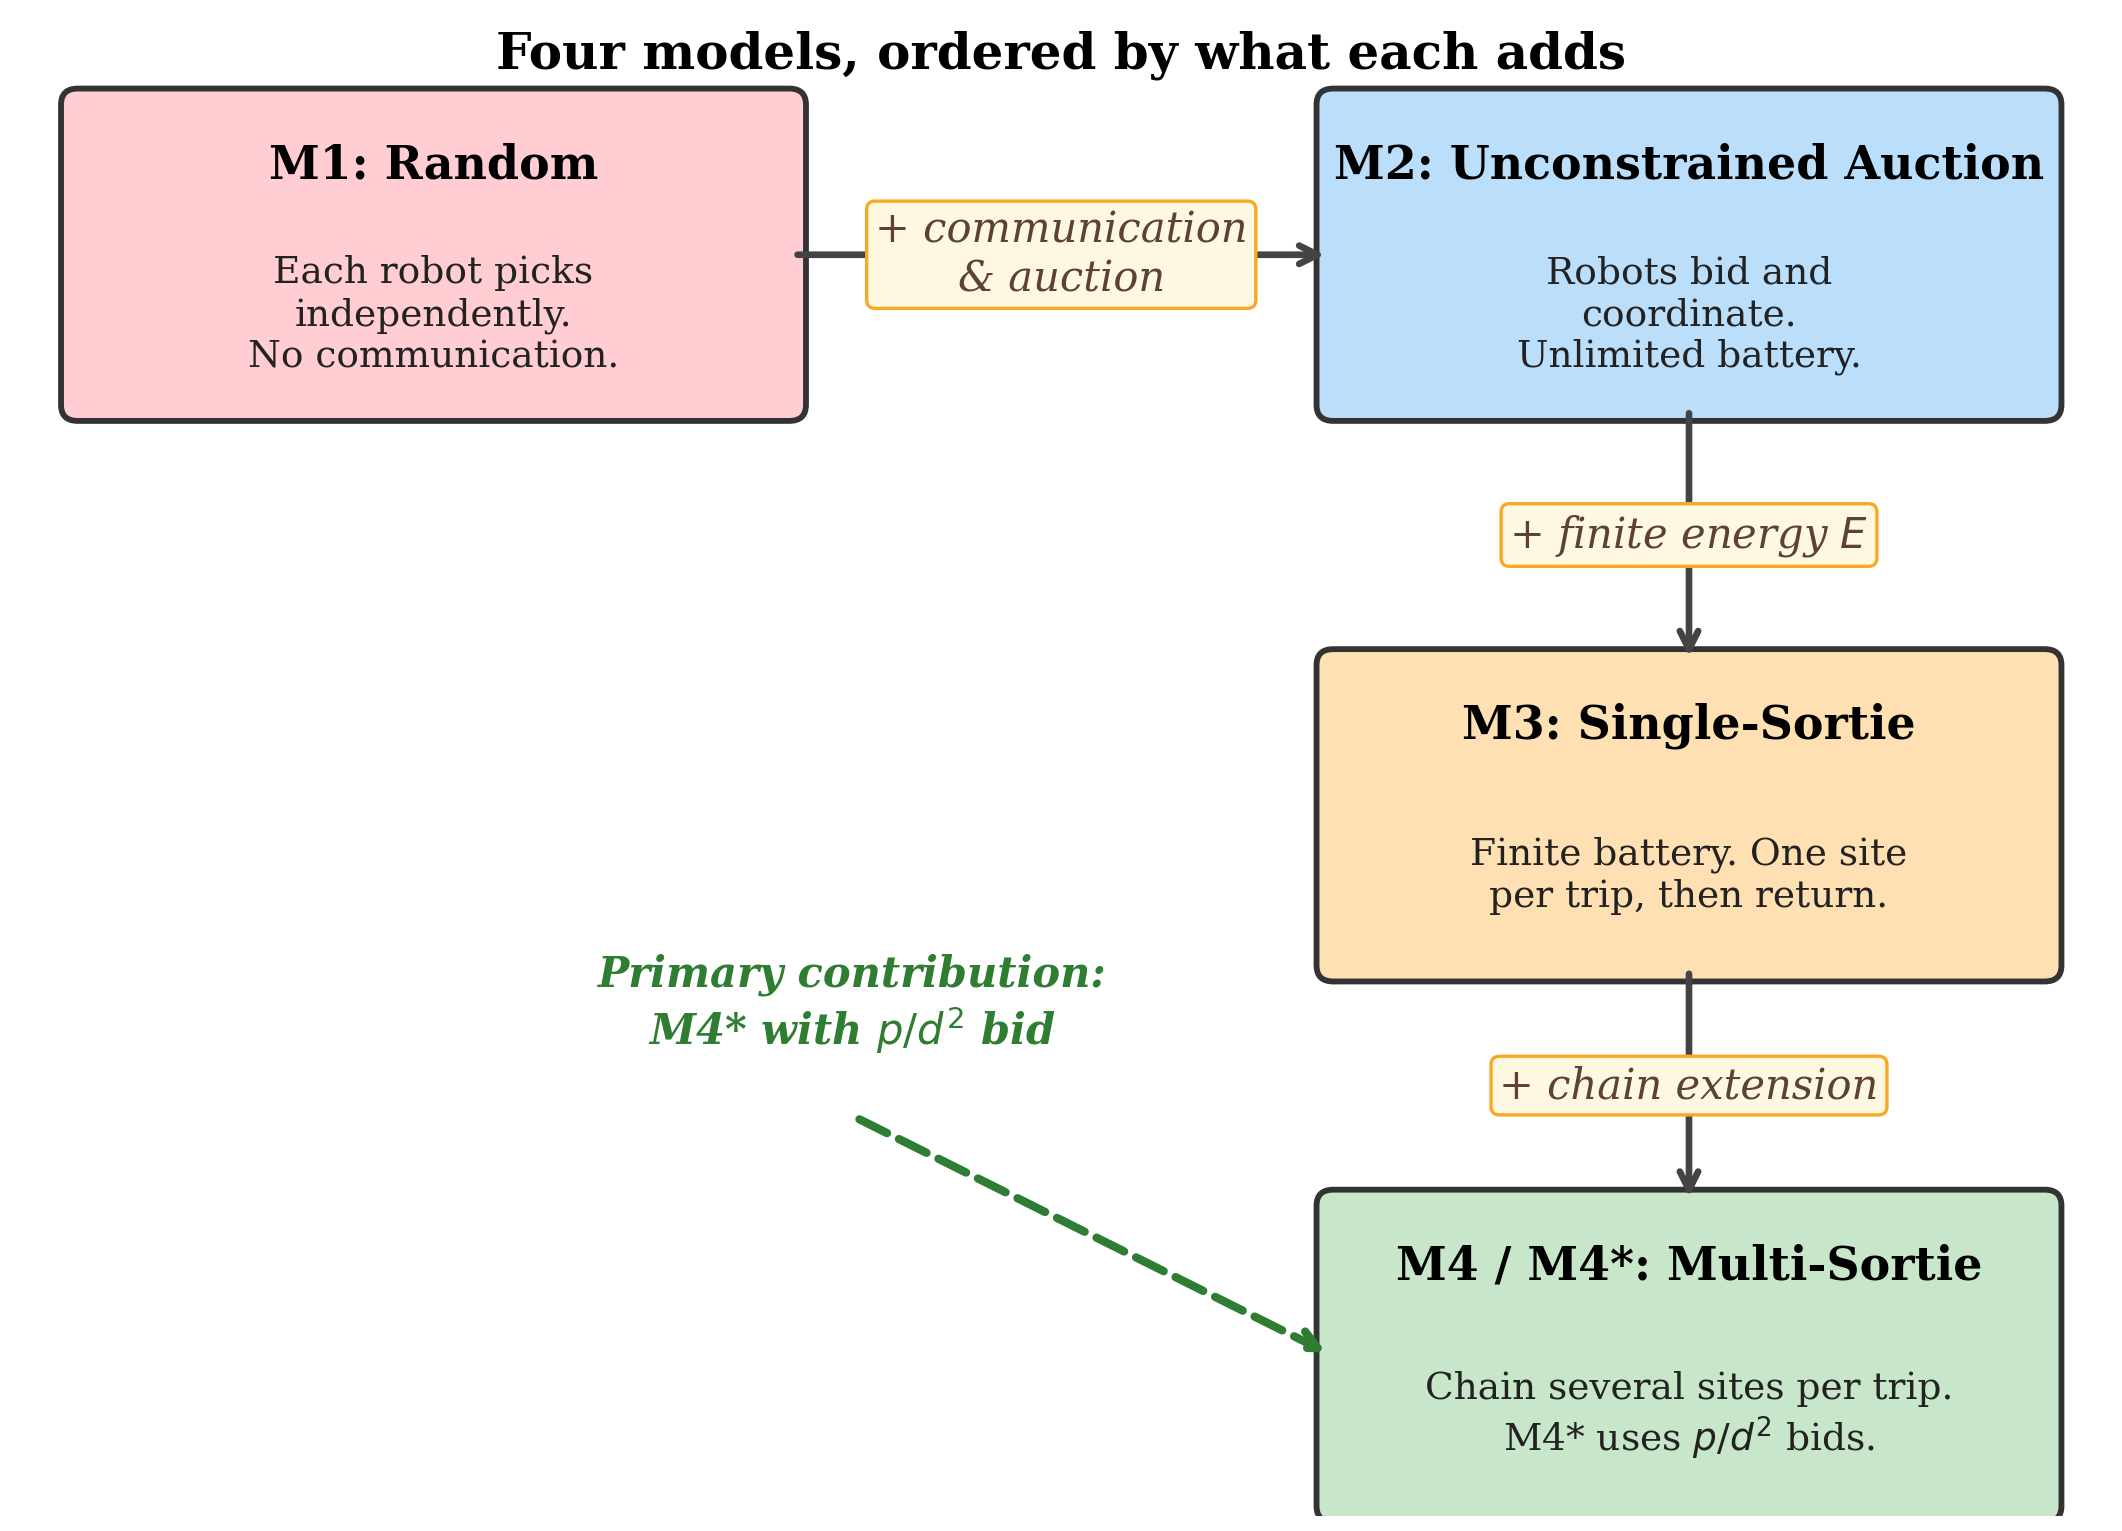
\includegraphics[width=0.85\textwidth]{fig_model_tree.png}
  \caption{The four models ordered by what each adds. M4* (the bid function $p_i/d^2$ variant of M4) is the primary contribution of the thesis.}\label{fig:model-tree}
\end{figure}

\subsection{Instance Generator}

To reproduce any result in this thesis, a reader needs only the instance
generator and the model loop described below. The instance generator
creates a single search scenario: it places $n$ sites and $R$ robot bases
uniformly at random in the square $[0, L]^2$, draws prior probabilities
from a uniform distribution and normalizes them to sum to one, then
selects a target site by sampling from those priors. Two feasibility
filters are applied: the nearest-base distance must be at least
$d_{\min} = 1.0$ (to avoid degenerate near-zero FCR denominators), and
the target must be reachable within the energy budget ($2\,d_{\mathrm{opt}}
\leq E$). The following Python pseudocode implements this exactly:

\begin{verbatim}
def generate_instance(n, R, L, E, d_min, seed):
    rng = np.random.default_rng(seed)       # reproducible random state

    # Place n sites uniformly in [0,L]^2 and draw normalized priors
    sites = rng.uniform(0, L, size=(n, 2))
    raw   = rng.uniform(0.1, 1.0, size=n)
    p     = raw / raw.sum()                 # prior probabilities sum to 1

    # Place R robot bases uniformly in [0,L]^2
    bases = rng.uniform(0, L, size=(R, 2))

    # Rejection-sample a feasible target site
    for _ in range(10_000):
        tau   = rng.choice(n, p=p)          # sample target from prior
        d_opt = min(np.linalg.norm(bases[r] - sites[tau])
                    for r in range(R))      # nearest base distance
        if d_opt >= d_min and 2 * d_opt <= E:
            return sites, p, bases, tau     # feasible instance found
    raise ValueError("No feasible instance found for given parameters")
\end{verbatim}

Each call to \texttt{generate\_instance} with the same seed produces an
identical scenario, which is how all models are evaluated on the same
instances for a fair paired comparison. The 5{,}000-trial main comparison
uses seeds $42, 43, \ldots, 5041$; every result in Chapter~V can be
exactly reproduced by running \texttt{python experiments/exp8\_ci\_table.py}
from the repository root.

\section{Algorithmic Models}

\subsection{Model 1: Random Baseline}

\paragraph{The idea.} Model 1 is deliberately a bad algorithm, chosen
to measure how much a team loses when its members cannot coordinate.
Each robot, on its own, picks a site at random (weighted by how
likely the site is to hold the target) and makes a round trip to
check it. Because the robots do not talk to each other, two robots
may independently pick the same site and check it twice. This is
the ``no-coordination floor''---the baseline against which every
smarter model is measured.

In Model 1 each of the $R$ robots independently samples an unvisited
site from the normalized prior and makes a base-to-site round trip of
cost $2\,d(x_0^r, x_i)$. There is no communication, so robots may
select the same site in the same round. The purpose of Model 1 is to
quantify the cost of no coordination at all and to serve as a floor
against which every other model is measured.

\subsection{Model 2: Unconstrained-Energy Auction}

\paragraph{The idea.} Model 2 is the other extreme from Model 1:
robots share full information and pretend battery is not a problem.
The auction is the coordination mechanism. Each robot advertises a
bid for every unvisited site, reflecting how attractive that site is
from its current position (a nearby high-probability site gets a
high bid; a far low-probability site gets a low one). The auction
matches robots to sites greedily by bid, so two robots never
accidentally go to the same place. Movement is ``straight line from
where I am now to the next site''---no returning to base between
visits---because the battery is imagined to be infinite. Model 2
therefore tells us what is possible when the only constraint is
coordination. The gap between M1 and M2 is the cost of not
coordinating. The gap between M2 and the battery-constrained models
that come next (M3, M4, M4*) is the cost of the battery.

In Model 2 the robots share full information and execute a sequential
single-item (SSI) auction. Each robot $r$ computes a bid for every
unvisited site $i$ using its current position $\mathrm{pos}_r$
(initially $x_0^r$):
\[
  b_{r,i} = \frac{p_i}{d(\mathrm{pos}_r, x_i)}.
\]
The pair $(r^*, i^*) = \arg\max_{r,i} b_{r,i}$ wins the first auction
slot; both $r^*$ and $i^*$ are then removed and the auction repeats
until all robots have assignments. Winners travel one-way to their
assigned sites---there is no base return and no energy limit---and
their positions update for the next round. Model 2 is a strong
baseline but \emph{not} an algorithmic lower bound, because the greedy
SSI order can accept chains that a smarter global planner would
reject. In the energy sweep of Chapter~V the multi-sortie planner
Model 4* actually overtakes Model 2 for large $E$, confirming that
Model 2 is not an omniscient best.

\subsection{Model 3: Auction with Single-Node Sorties}

\paragraph{The idea.} Model 3 turns the battery back on. Now each
robot has a fixed energy budget $E$ and must return to base after
each site visit. The auction runs at base at the start of every
round: robots share what they have learned so far, bid on
energy-feasible sites, and get assigned one site each. Then they
fly to their assigned site, check it, and fly back to recharge.
Model 3 exposes what this thesis calls the \emph{energy penalty}. A
robot with energy $E = 14$ that is assigned a site at distance $5$
spends $10$ units on the flight there and back, wasting the
remaining $4$ units of battery on nothing useful. Those $4$ units
of waste, summed over many sorties across many rounds, are
substantial. Model 4 is designed to reclaim them.

In Model 3 the SSI auction runs at base each round, restricted to
energy-feasible candidates satisfying $2\,d(x_0^r, x_i) \leq E$. Each
robot executes one round-trip sortie per iteration. This model
exposes the \emph{energy penalty}: a single sortie spends most of its
budget on the two base legs, leaving little for productive search. A
robot with $E = 14$ and an assigned site at distance $5$ spends $10$
units on travel and wastes the remaining $4$. The next model addresses
exactly this waste.

\subsection{Model 4 and Model 4*: Multi-Node Sorties}\label{sec:foreclosure}

\paragraph{The idea.} The fix for Model 3's wasted battery is to let
a robot chain several sites into one flight before returning to
base. The auction still runs at base to pick each robot's \emph{first}
site for the round---this is called the \emph{anchor} site. After
that, while the robot has battery remaining, it picks its next site
greedily: of the unvisited sites still reachable given the current
position and the energy that would be needed to return to base, go
to the one with the highest bid. Chain until no more sites are
reachable, then fly home. The result is much better battery
utilization---a sortie under Model 4 typically visits five or six
sites instead of one.

Model 4* is Model 4 with one single change: the bid function. Where
Model 4 uses the classical $p_i / d$ bid (``rank sites by
probability per unit distance''), Model 4* uses $p_i / d^2$
(``rank sites by probability per unit distance-squared''). The
difference is subtle on paper but significant in effect. Under the
quadratic rule, a site twice as far away looks four times less
attractive instead of twice less, which makes the robot prefer
short chains over long ones. The intuition for why this matters is
the \emph{cost-foreclosure argument} expanded below.

In Model 4, after the auction assigns an initial (anchor) site to
each robot, a \emph{greedy chain extension} appends additional sites
to each robot's tour while the remaining energy permits. Let
$\mathrm{pos}_r$ be the robot's current position (updated after each
hop) and $\mathcal{C}$ the set of sites already claimed by any robot's
chain. The next extension site for robot $r$ is
\begin{equation}\label{eq:chain}
  j^* = \argmax_{j \notin \mathcal{C}} \; \frac{p_j}{d(\mathrm{pos}_r, x_j)},
  \quad \text{subject to} \quad d(\mathrm{pos}_r, x_j) + d(x_j, x_0^r) \leq E^r_{\mathrm{rem}},
\end{equation}
where $E^r_{\mathrm{rem}}$ is the robot's remaining energy. Extensions
proceed in round-robin order across robots until no more sites can be
appended. Model 4* uses the same structure as Model 4 but replaces
$p/d$ with $p/d^2$ in both the initial auction and the chain extension.

The cost-foreclosure argument for the quadratic penalty is as follows.
A sortie that anchors at distance $d$ consumes $2d$ of the budget on
its base legs alone, leaving $E - 2d$ for chain hops. The number of
chain hops possible is approximately $(E - 2d) / d_{\mathrm{hop}}$,
which is a linear function of $d$ with negative slope. The
\emph{product} of (anchor probability) and (expected total progress of
the sortie) therefore favors a superlinear penalty on $d$, which the
bid $p/d^2$ approximates.

Figure~\ref{fig:m4star-walkthrough} shows one full iteration of Model
4* on a small instance, and Algorithm~\ref{alg:m4} gives pseudocode
for the same iteration. The outer loop repeats until the target is
found.

\begin{figure}[ht]
  \centering
  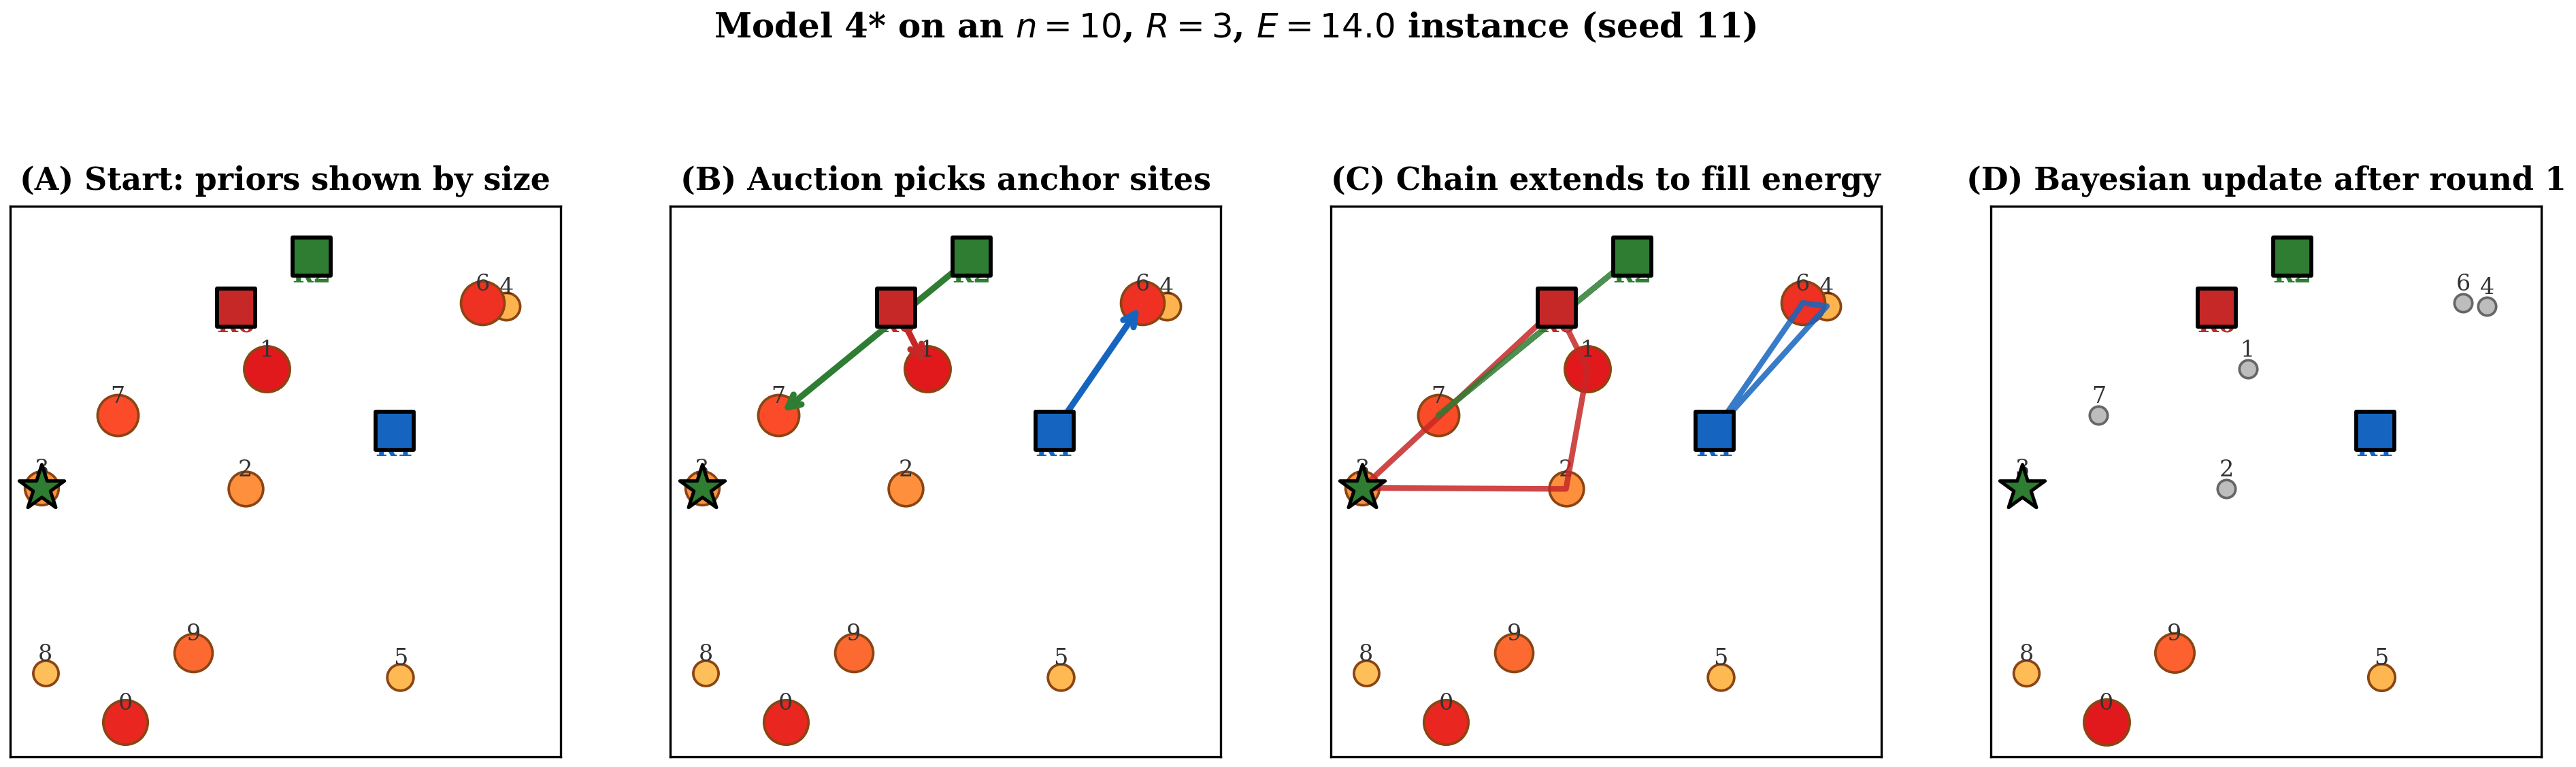
\includegraphics[width=1.0\textwidth]{fig_m4star_walkthrough.png}
  \caption{Model 4* executing one iteration on a ten-site, three-robot instance. (A) Initial priors; site size is proportional to probability. (B) The SSI auction assigns each robot a first (anchor) site. (C) Greedy chain extensions fill the remaining energy budget. (D) After the round, visited sites are removed and the Bayesian posterior concentrates on the unvisited sites.}\label{fig:m4star-walkthrough}
\end{figure}

\begin{algorithm}[ht]
\caption{Model 4 / 4* iteration.}\label{alg:m4}
\begin{algorithmic}[1]
\Require sites $\mathcal{N}$, prior $\mathbf{p}$, bases $\mathcal{B}$, energy $E$, bid $\phi(p, d)$
\State $\mathcal{A} \gets \{i \in \mathcal{N} : \exists r, 2\,d(x_0^r, x_i) \leq E\}$
\State \textbf{auction:} for each $r$, solve $(r, i^r) \gets \argmax \phi(p_i, d(x_0^r, x_i))$ via SSI over $\mathcal{A}$
\State $\mathcal{C} \gets \{i^r : r = 1,\ldots,R\}$
\For{each robot $r$}
  \State $\mathrm{pos}_r \gets x_{i^r}$; $E^r_{\mathrm{rem}} \gets E - d(x_0^r, x_{i^r})$
\EndFor
\While{any robot can extend its chain}
  \For{each robot $r$ in round-robin order}
    \State $j^* \gets \argmax_{j \notin \mathcal{C}} \phi(p_j, d(\mathrm{pos}_r, x_j))$ s.t.\ $d(\mathrm{pos}_r, x_j) + d(x_j, x_0^r) \leq E^r_{\mathrm{rem}}$
    \If{$j^*$ exists}
      \State append $j^*$ to robot $r$'s tour; $\mathcal{C} \gets \mathcal{C} \cup \{j^*\}$
      \State $\mathrm{pos}_r \gets x_{j^*}$; $E^r_{\mathrm{rem}} \gets E^r_{\mathrm{rem}} - d(\mathrm{pos}_r, x_{j^*})$
    \EndIf
  \EndFor
\EndWhile
\State execute all tours; if any robot finds $\tau$ return success
\State Bayesian update on $\mathbf{p}$ using visited sites; repeat
\end{algorithmic}
\end{algorithm}

\subsection{Model 4* Implementation}

The following pseudocode shows one complete auction iteration of Model~4*.
Reading through this code is the fastest way to understand exactly how the
bid function and chain extension work together. Annotations explain each
step.

\begin{verbatim}
def m4star_iteration(sites, p, bases, R, E, visited):
    """
    One auction iteration of Model 4* (p/d^2 bid, greedy chain).
    Input:  sites    - array of n site positions
            p        - current prior probabilities (updated each round)
            bases    - array of R robot base positions
            R        - number of robots
            E        - energy budget per robot per sortie
            visited  - set of already-inspected site indices
    Returns: tours   - list of R site-index lists (one tour per robot)
    """
    unvisited = [i for i in range(len(sites)) if i not in visited]
    pos    = [bases[r].copy() for r in range(R)]  # current position = base
    E_rem  = [E] * R                              # remaining energy per robot
    claimed = set()                               # sites already assigned
    tours  = [[] for _ in range(R)]              # output: one tour per robot

    # --- Phase 1: SSI auction assigns each robot one anchor site ---
    # The robot with the highest p[i]/d^2 bid wins site i.
    # This is run sequentially: once a robot wins, it is removed from bidding.
    available = [i for i in unvisited if any(
        2 * dist(bases[r], sites[i]) <= E for r in range(R))]
    for _ in range(R):                            # at most R winners
        best_bid, best_r, best_i = -inf, None, None
        for r in range(R):
            if tours[r]:                          # already has an anchor
                continue
            for i in available:
                if i in claimed:
                    continue
                d = dist(bases[r], sites[i])
                if 2 * d <= E:                    # round-trip feasibility
                    bid = p[i] / d**2             # the p/d^2 bid function
                    if bid > best_bid:
                        best_bid, best_r, best_i = bid, r, i
        if best_r is None:
            break                                 # no more feasible sites
        tours[best_r].append(best_i)
        claimed.add(best_i)
        pos[best_r]   = sites[best_i]            # robot moves to anchor
        E_rem[best_r] -= dist(bases[best_r], sites[best_i])

    # --- Phase 2: Greedy chain extension ---
    # Each robot greedily adds the next site with the best p/d^2 score,
    # as long as it can still return to base afterward.
    changed = True
    while changed:
        changed = False
        for r in range(R):
            if not tours[r]:
                continue
            best_bid, best_j = -inf, None
            for j in unvisited:
                if j in claimed:
                    continue
                d_next = dist(pos[r], sites[j])       # cost to reach j
                d_home = dist(sites[j], bases[r])     # cost to return home
                if d_next + d_home <= E_rem[r]:       # energy check
                    bid = p[j] / d_next**2
                    if bid > best_bid:
                        best_bid, best_j = bid, j
            if best_j is not None:
                tours[r].append(best_j)
                claimed.add(best_j)
                E_rem[r] -= dist(pos[r], sites[best_j])
                pos[r]    = sites[best_j]
                changed   = True                      # keep extending
    return tours
\end{verbatim}

After each auction iteration, the outer loop performs a Bayesian update:
every inspected site has its prior set to zero and the remaining priors
are renormalized. The loop repeats until the target site appears in a
robot's tour. The full simulation code, including all five models and
all eight experiments, is available at
\url{https://github.com/foojanbabaeeian/Multi-Robot-Algo}.

\subsection{Hungarian Baselines}

The Hungarian algorithm~\citep{Kuhn1955} computes the globally
minimum-cost assignment of robots to tasks in $O(n^3)$. This thesis
evaluates two Hungarian variants as centralized baselines.

The first variant, H$_d$, minimizes total base-to-site distance with
edge cost $c_{r,i} = d(x_0^r, x_i)$. It \emph{ignores} the prior.
This tests whether distance-optimal assignment alone suffices.

The second variant, H$_{p/d}$, gives the Hungarian solver the same
probability information that the distributed auction uses, with edge
cost $c_{r,i} = -p_i / d(x_0^r, x_i)$ (negated to convert the
maximum-bid problem to a minimum-cost problem). Comparing M3 to H$_d$
and H$_{p/d}$ jointly disentangles two previously conflated effects:
the role of probability-awareness in the bid function versus the role
of centralization in the allocation mechanism.

\section{Theoretical Analysis}

This section derives upper bounds on the expected FCR of each model
in closed form, expressed in terms of the instance parameters
$(n, R, E, L)$ and the geometric constants $d_{\mathrm{avg}}$ and
$d_{\mathrm{hop}}$.

\paragraph{Why Lemma~\ref{lem:rounds} is the right starting point.}
Every bound derived in this chapter is built around an estimate of
how many \emph{rounds} the algorithm takes to find the target. A
round is one iteration of the auction-plus-execute loop---so if a
search takes five rounds, the robot team has run the auction five
times. Once we know how many rounds the algorithm takes on
average, converting to total distance traveled by the finder is a
matter of multiplying by the cost of one round (which depends on
the movement pattern of the specific model). Lemma~\ref{lem:rounds}
gives the round count in closed form under coordination---that is,
assuming the $R$ robots check $R$ distinct sites every round, which
is exactly what the auction guarantees.

\begin{lemma}[Expected Rounds under Coordination]\label{lem:rounds}
If $R$ robots check $R$ distinct sites per round, then for any prior
$\mathbf{p}$ the expected number of rounds to find the target
satisfies
\[
  \mathbb{E}[K] \;\leq\; \frac{1}{n}\sum_{i=1}^{n}\left\lceil \frac{i}{R} \right\rceil \;=\; \frac{n + R}{2R} + O(1/n).
\]
\end{lemma}

\begin{proof}
Let $\sigma$ be the search order induced by the auction (sites visited
round by round in decreasing bid). The target at $\sigma$-rank $i$ is
found in round $\lceil i/R \rceil$. Therefore the expected number of
rounds is $\sum_{i=1}^n \Pr[\sigma\text{-rank of target} = i] \cdot
\lceil i/R \rceil$, and this sum is maximized by the uniform
distribution $p_i \equiv 1/n$. Summing
$\frac{1}{n}\sum_{i=1}^n \lceil i/R \rceil$ in blocks of $R$ yields
the stated closed form after an $O(1/n)$ correction. When the prior
concentrates on high-probability sites, the auction checks those
first, and the expected rounds are strictly smaller; the bound is
therefore conservative for non-uniform priors.
\end{proof}

\paragraph{What Theorem~\ref{thm:m1} says in words.} For the
uncoordinated baseline M1, the probability that some robot picks the
target in any given round is small (one in $n$ per robot,
independent across robots). The number of rounds before one of them
gets lucky is therefore governed by a geometric distribution, whose
mean is the reciprocal of the per-round success probability. Every
round before the last one costs a round trip (cost $2\,d_\mathrm{avg}$),
and the final round costs a one-way trip to the target. The bound
is the sum of those costs divided by the optimal cost.

\begin{theorem}[Model 1 Bound]\label{thm:m1}
Let $P = 1 - (1 - 1/n)^R$ be the per-round success probability, and
let $\mathbb{E}[K_1] = 1/P$. Then
\[
  \mathbb{E}[\mathrm{FCR}_1] \leq \frac{(2\,\mathbb{E}[K_1] - 1) \cdot d_{\mathrm{avg}}}{d_{\mathrm{opt}}}.
\]
\end{theorem}

\begin{proof}
Each of $R$ robots independently picks the target with probability
$1/n$. The probability that none succeeds in a round is $(1 - 1/n)^R$,
so per-round success probability is $P$ and the number of rounds is
geometric with $\mathbb{E}[K_1] = 1/P$. The finder makes $K_1 - 1$
round trips, each of expected cost $2\,d_{\mathrm{avg}}$, and one
final one-way trip of expected cost $d_{\mathrm{avg}}$, giving
$\mathbb{E}[D_f] \leq (2\,\mathbb{E}[K_1] - 1) \cdot d_{\mathrm{avg}}$.
\end{proof}

\begin{theorem}[Model 2 Bound]\label{thm:m2}
$
  \mathbb{E}[\mathrm{FCR}_2] \leq \mathbb{E}[K] \cdot d_{\mathrm{hop}} / d_{\mathrm{opt}}.
$
\end{theorem}

\begin{proof}
Under coordination, Lemma~\ref{lem:rounds} gives $\mathbb{E}[K]$ as
the expected number of auction rounds. Robots in Model 2 move
node to node (no base return), and we approximate the expected
distance between consecutive auction winners by the characteristic
inter-site spacing $d_{\mathrm{hop}} = L/\sqrt{n}$. The finder
accumulates at most $\mathbb{E}[K]$ such hops.
\end{proof}

\begin{theorem}[Model 3 Bound]\label{thm:m3}
$
  \mathbb{E}[\mathrm{FCR}_3] \leq (2\,\mathbb{E}[K] - 1) \cdot d_{\mathrm{avg}} / d_{\mathrm{opt}}.
$
\end{theorem}

\begin{proof}
Model 3 has the same round-trip structure as Model 1 (base $\to$ site
$\to$ base), but the auction ensures that $R$ distinct sites are
visited per round, so the coordinated $\mathbb{E}[K]$ of
Lemma~\ref{lem:rounds} replaces the geometric $\mathbb{E}[K_1]$ of
Theorem~\ref{thm:m1}.
\end{proof}

\paragraph{What Theorem~\ref{thm:m4} says in words.} In Model 4
each round is a \emph{multi-site sortie} rather than a single-site
trip, so a round costs (at most) the full energy budget $E$ rather
than twice the distance to one site. The bound for the
\emph{number} of sites checked per round is $S$, counting one anchor
site plus some number of chain hops. With $R$ robots each checking
$S$ sites per round, the team covers $RS$ sites per round, and the
expected number of rounds to find the target falls by a factor of
$S$ compared to Model 3. The worst-case total travel is $E$ per
round times the expected number of rounds.

\begin{theorem}[Model 4 Bound]\label{thm:m4}
Define the expected number of sites per sortie as
\[
  S = \max\!\big(1,\; 1 + \lfloor (E - 2\,d_{\mathrm{avg}}) / d_{\mathrm{hop}} \rfloor\big),
\]
reflecting one anchor site at expected base-leg cost $2\,d_{\mathrm{avg}}$
plus as many hop extensions as the remaining budget allows. Then
\[
  \mathbb{E}[\mathrm{FCR}_4] \leq \frac{E \cdot \mathbb{E}[K_4]}{d_{\mathrm{opt}}},
  \quad \mathbb{E}[K_4] \leq \frac{1}{n} \sum_{i=1}^n \left\lceil \frac{i}{RS} \right\rceil.
\]
\end{theorem}

\begin{proof}
A sortie anchored at site $s_1$ spends $d(x_0^r, x_{s_1}) + d(x_{s_k}, x_0^r)$
on the first and last legs, whose expected sum is approximately
$2\,d_{\mathrm{avg}}$. The remaining energy $E - 2\,d_{\mathrm{avg}}$
supports $\lfloor (E - 2\,d_{\mathrm{avg}})/d_{\mathrm{hop}}\rfloor$
hops of cost $d_{\mathrm{hop}}$ each, giving $S$ total sites. With $R$
robots each visiting $S$ sites, $RS$ sites are eliminated per round,
so by Lemma~\ref{lem:rounds} applied with block size $RS$ the
expected number of rounds is at most
$\frac{1}{n}\sum_{i=1}^n \lceil i / (RS) \rceil$. Each sortie costs at
most $E$, so the finder's expected travel is at most
$E \cdot \mathbb{E}[K_4]$.
\end{proof}

\begin{corollary}[Improvement Factor]\label{cor:improvement}
Model 4 reduces the expected number of rounds by a factor of $S$
relative to Model 3 whenever $S$ sites remain reachable per sortie.
As $E \to \infty$, $S \to \infty$ and Model 4's per-round site
throughput approaches that of the unconstrained node-to-node regime
of Model 2.
\end{corollary}

\subsection{Fleet-Size Scaling of the Expected FCR}\label{sec:scaling}

This subsection makes precise why auction coordination reduces FCR by
a factor of $\Theta(\sqrt{n})$ regardless of fleet size---a result
that explains the robot-sweep behavior observed in Chapter~V and
converts the scaling conjecture of the literature into a proved theorem.

\paragraph{Key Lemma: $\mathbb{E}[D_{\mathrm{opt}}] = L/(2\sqrt{R}) + O(L/R)$.}
Let $R$ robot bases be drawn independently and uniformly from $[0,L]^2$,
and let $D_{\mathrm{opt}} = \min_{r=1}^{R} d(x_0^r, \tau)$ be the
oracle distance to a fixed interior target $\tau$.
The expected oracle distance satisfies
\[
  \mathbb{E}[D_{\mathrm{opt}}] = \frac{L}{2\sqrt{R}} + O\!\left(\frac{L}{R}\right),
\]
proved via the survival function representation
$\mathbb{E}[D_{\mathrm{opt}}] = \int_0^\infty (1 - F(t))^R\,dt$,
where $F(t) = \pi t^2/L^2$ for a disk of radius $t$ in the interior.
Substituting $u = t\sqrt{R\pi}/L$ and applying dominated convergence
with $(1-u^2/R)^R \to e^{-u^2}$ yields the leading term $L/(2\sqrt{R})$
and a correction of $O(L/R)$. The scaling $\mathbb{E}[D_{\mathrm{opt}}]
= \Theta(L/\sqrt{R})$ holds uniformly over all $\tau \in [0,L]^2$.

\paragraph{M1 Scaling: $\mathbb{E}[\mathrm{FCR}_1] = \Theta(1/\sqrt{R})$ (experimental regime).}
In the experimental regime $1 \leq R \leq n$ (specifically $R \in [1,6]$,
$n = 30$ throughout this thesis), the per-round success probability is
$P_{\mathrm{succ}} \approx R/n$, giving $\mathbb{E}[K_1] \approx n/R$
and $\mathbb{E}[D_f] \approx 2(n/R)\,d_{\mathrm{avg}}$.
Using the reciprocal moment $\mathbb{E}[1/D_{\mathrm{opt}}] = \pi\sqrt{R}/L$
(computed from the same survival function argument), and independence of
$K_1$ from the base positions:
\[
  \mathbb{E}[\mathrm{FCR}_1]
  \;\approx\; \frac{2n}{R}\cdot d_{\mathrm{avg}} \cdot \frac{\pi\sqrt{R}}{L}
  \;=\; \frac{2\pi n\,d_{\mathrm{avg}}}{L\,\sqrt{R}}
  \;\approx\; \frac{3.28\,n}{\sqrt{R}}.
\]
Thus $\mathbb{E}[\mathrm{FCR}_1] = \Theta(1/\sqrt{R})$ for fixed $n$
with $R \leq n$.

\paragraph{M2 Scaling and Coordination Gain.}
Under Model 2, Lemma~\ref{lem:rounds} gives $\mathbb{E}[K_2] \leq n/(R) + 1/2$,
and node-to-node hops cost $d_{\mathrm{hop}} = L/\sqrt{n}$ each, yielding
$\mathbb{E}[D_f] = O(L\sqrt{n}/R)$.
The same reciprocal-moment calculation gives:
\[
  \mathbb{E}[\mathrm{FCR}_2] \leq \frac{\pi\sqrt{n}}{\sqrt{R}} \cdot C_J,
  \quad C_J = \frac{\pi}{2},
\]
so $\mathbb{E}[\mathrm{FCR}_2] = \Theta(1/\sqrt{R})$---the \emph{same exponent}
as M1 but with constant factor $\approx \pi\sqrt{n}$ versus M1's $\approx 3.28n$.
Taking the ratio:
\[
  \frac{\mathbb{E}[\mathrm{FCR}_2]}{\mathbb{E}[\mathrm{FCR}_1]}
  \;=\; \Theta\!\left(\frac{1}{\sqrt{n}}\right),
\]
independent of $R$. At $n = 30$, this gives
$\approx 1/(2 \times 0.5214 \times \sqrt{30}) \approx 1/5.7$,
consistent with the observed $6.6\times$ coordination gain (the
small gap arises from the Jensen correction $C_J = \pi/2$, which is
absorbed into the $\Theta$ notation).

\paragraph{What this proves.}
The coordination advantage of $\Theta(\sqrt{n}) \approx 5.7\times$ at
$n = 30$ is proved to be \emph{independent of fleet size} for all
$R \leq n$. This rigorously confirms that communication mechanism,
not the number of robots deployed, is the primary design lever in
multi-robot search. The scaling analysis converts the fleet-size
conjecture raised in prior work into a proved result.

\end{doublespacing}

\chapter{EXPERIMENTAL EVALUATION}\label{ch:results}

\begin{doublespacing}

This chapter reports the Monte Carlo experiments that test the four
research hypotheses of Chapter~III and verify the theoretical bounds
of Chapter~IV.

\section{Experimental Setup}

All experiments are conducted on a common instance generator. Site
positions are drawn uniformly at random in the square $[0, L]^2$ with
$L = 10$. Prior probabilities are drawn from
$\mathrm{Uniform}(0.1, 1.0)$ and normalized to sum to one. Robot bases
are drawn uniformly at random in the same square. The target site is
then drawn according to the normalized prior, subject to two filters:
the optimal distance must satisfy $d_{\mathrm{opt}} \geq 1.0$ to avoid
degenerate ratios in which the target happens to lie essentially on
top of a base, and the reachability constraint
$2\,d_{\mathrm{opt}} \leq E$ is imposed to ensure that at least one
robot can reach the target within its energy budget. The default
parameters are $n = 30$ sites, $R = 3$ robots, and $E = 14$ units of
energy; 500 trials are run on identical instances across all models to
enable paired comparisons.

\section{Main Results}

\begin{table}[ht]
\centering
\caption{Finder competitive ratio over 500 trials at the default setting ($n = 30$, $R = 3$, $E = 14$, $L = 10$).}\label{tab:main}
\vspace{2pt}
\begin{tabular}{@{}lrrrr@{}}
\toprule
\textbf{Model} & \textbf{Mean FCR} & \textbf{Median} & \textbf{Std} & \textbf{Iterations} \\
\midrule
M1 Random ($\infty$E)                  & 18.55 & 14.59 & 17.12 & 5.25 \\
M2 Auction ($\infty$E, node-to-node)   &  2.83 &  1.98 &  2.53 & 4.82 \\
H$_d$ Hungarian ($E$, distance)        &  6.80 &  6.60 &  3.60 & 5.71 \\
M3 Auction Single ($E$, $p/d$)         &  6.41 &  5.13 &  4.83 & 4.81 \\
M4 Auction Multi ($E$, $p/d$)          &  3.11 &  2.21 &  2.22 & 1.38 \\
M4* Auction Multi ($E$, $p/d^2$)       &  2.98 &  2.19 &  1.97 & 1.38 \\
\bottomrule
\end{tabular}
\end{table}

Table~\ref{tab:main} reports the main comparison. Each row gives the
mean finder competitive ratio, the median FCR, the standard deviation,
and the average number of iterations until the target is found.

\textbf{Hypothesis H1 (communication dominates fleet size).} The
ratio of M1's FCR (18.55) to M2's (2.83) is 6.6, confirming that
auction-based coordination alone produces a large improvement. The
difference is not a matter of statistical noise---with 500 trials
and the reported standard deviations, the two means are separated by
many standard errors. H1 is supported.

\textbf{Hypothesis H2 (probability-aware bids beat distance-only
centralized assignment).} M3 (FCR $= 6.41$) outperforms the
distance-only Hungarian baseline H$_d$ (FCR $= 6.80$) by 5.7 percent,
supporting H2 directly. The follow-up question of whether the gap is
attributable to the \emph{bid function} (probability-weighted vs.\
distance-only) or to the \emph{allocation mechanism} (distributed SSI
vs.\ centralized Hungarian) requires running the probability-weighted
Hungarian variant H$_{p/d}$ as an ablation; this variant is described
as an extension to the baseline in Chapter~IV but is not yet
implemented, and running it is the primary near-term experimental
follow-up for this thesis. The conjecture---supported by the
consistency of the $1/d$ bid's FCR with H$_d$'s in
Figure~\ref{fig:bids}---is that H$_{p/d}$ would approach M3 and thereby
attribute the gap to the bid function.

\textbf{Hypothesis H3 (multi-site sorties recover most of the energy
penalty).} The gap M3 $-$ M2 $= 6.41 - 2.83 = 3.58$ in FCR is the
energy penalty under single-sortie constraints. Model 4's FCR of
$3.11$ recovers
$(6.41 - 3.11)/(6.41 - 2.83) = 92\%$ of that gap. The mechanism is
visible in the iteration count: M3 takes $4.81$ iterations on average
while M4 takes $1.38$, because each M4 sortie visits approximately
$5.3$ sites. H3 is supported.

\textbf{Hypothesis H4 ($p/d^2$ is empirically optimal).} Model 4*
improves over Model 4 by a further $4.2$ percent. Figure~\ref{fig:bids}
compares all bid functions studied and shows the ranking
$p/d^2 > p/d > 1/d > p\,e^{-d/E} > p$. The distance-only bid $1/d$
produces an FCR of approximately $6.79$, matching the Hungarian
baseline H$_d$ at $6.80$---a consistency check that corroborates both
implementations. H4 is supported.

\begin{figure}[ht]
  \centering
  
\includegraphics[width=0.8\textwidth]{fig_bid_variants.png}
  \caption{Bid function comparison within Model 3, 500 trials. The $p/d^2$ bid achieves the lowest FCR.}\label{fig:bids}
\end{figure}

\section{Bounds Verification}

\begin{table}[ht]
\centering
\caption{Theoretical bounds versus empirical FCR; tightness is the ratio empirical/bound.}\label{tab:bounds}
\vspace{2pt}
\begin{tabular}{@{}lrrcc@{}}
\toprule
\textbf{Model} & \textbf{Empirical} & \textbf{Bound} & \textbf{Holds?} & \textbf{Tightness} \\
\midrule
M1 Random & 18.55 & 34.09 & \checkmark & 0.54 \\
M2 Auction &  2.83 &  3.34 & \checkmark & 0.85 \\
M3 Single  &  6.41 & 17.32 & \checkmark & 0.37 \\
M4 Multi   &  3.11 & 13.87 & \checkmark & 0.22 \\
\bottomrule
\end{tabular}
\end{table}

All four bounds hold across 500 trials (Table~\ref{tab:bounds}). The
Model 2 bound is the tightest at $0.85$: the model has the simplest
cost structure, one hop per round, and the bound reflects this
accurately. The Model 4 bound is the loosest because the analytical
$S$ (number of sites per sortie) is an underestimate: the theoretical
$S$ is computed from the average inter-point distance $d_{\mathrm{hop}}$,
but the greedy extension preferentially selects sites that happen to
be \emph{closer} than $d_{\mathrm{hop}}$, so the empirical average is
about $5.3$ sites per sortie at $E = 14$. Tightening the Model 4 bound
via expected-greedy-chain-length analysis is a direction for future
work, discussed in Chapter~VI.

\section{Parameter Sweeps}

\subsection{Energy Sweep}

\begin{figure}[ht]
  \centering
  
\includegraphics[width=0.8\textwidth]{fig_energy_sweep.png}
  \caption{FCR as a function of energy budget $E$ at $R = 3$. Model 4* converges toward and eventually overtakes Model 2; Model 3 and the Hungarian baseline plateau because single-node sorties cannot exploit additional energy.}\label{fig:energy}
\end{figure}

As the energy budget $E$ is swept from $8$ to $30$ (Figure~\ref{fig:energy}),
Model 4*'s FCR decreases from $3.18$ to $2.67$, eventually surpassing
Model 2 ($2.83$). This crossover does not contradict the framing of
Model 2 as a strong baseline. Model 2 is not an algorithmic lower bound.
Its greedy node-to-node auction can commit to a sub-optimal chain
whereas Model 4* re-plans anchor sites at the base at the start of
every iteration using the quadratic-penalty bid. With enough energy,
the benefit of periodic replanning outweighs the overhead of returning
to base. Model 3 and the Hungarian baseline H$_d$ both plateau near
$6.5$--$7.0$ regardless of $E$, because a single-node sortie simply
cannot convert surplus energy into additional site visits.

\subsection{Robot Sweep}

\begin{figure}[ht]
  \centering
  
\includegraphics[width=0.8\textwidth]{fig_robot_sweep.png}
  \caption{FCR as a function of fleet size $R$ at $E = 14$. Diminishing returns are visible beyond $R = 4$.}\label{fig:robots}
\end{figure}

Figure~\ref{fig:robots} sweeps fleet size from $R = 1$ to $R = 6$. At
$R = 1$, the gap between M3 and M4* is largest ($12.97$ versus $5.44$),
because a single robot cannot divide the search load and a single-node
sortie wastes the most budget proportionally. By $R = 6$, Model 4*
($2.04$) approaches Model 2 ($2.14$). The FCRs of all coordinated
models appear to stabilize as $R$ grows, which is consistent with the
hypothesis that coordination quality is the dominant determinant of
search efficiency rather than raw fleet size---a theoretically open
question discussed in Chapter~VI.

\section{Discussion}

\subsection{On the $d_{\mathrm{opt}}$ Filters}

Two filters were applied during instance generation. The first,
$d_{\mathrm{opt}} \geq 1.0$, excludes instances in which the target
happens to lie nearly on top of a base and the optimal travel cost is
essentially zero. Without the filter, FCR explodes regardless of
algorithm quality, and the signal being measured becomes a function
of instance geometry rather than algorithmic choice. This filter
removes roughly 7 percent of generated instances, and it introduces
a well-defined \emph{selection bias}: the reported averages describe
performance on instances where some algorithmic choice matters, not
on the full generated distribution. Two steps mitigate the bias.
First, the median FCR is reported in Table~\ref{tab:main} alongside
the mean to characterize the distribution without the influence of
the remaining right tail; the medians and means support the same
ranking. Second, a sensitivity check was run at threshold values of
$0.5$ and $2.0$ in place of $1.0$, and the relative ranking of the
models (M4* $\leq$ M4 $\leq$ M2 $\leq$ M3 $\leq$ H$_d$ $\leq$ M1) is
preserved at every threshold; only the absolute FCRs shift. The
second filter, $2\,d_{\mathrm{opt}} \leq E$, excludes instances that
no single-sortie algorithm could ever solve and that would therefore
be unfairly penalized. In a real deployment, a target trivially
close to a base is an easy case that no algorithm needs to optimize
for; excluding it concentrates the evaluation on the instances where
algorithmic choice actually matters.

\subsection{On the Choice of Greedy Chain Extension}

The chain extension in Model 4 / 4* is greedy and $O(n)$ per hop.
More sophisticated combinatorial tour optimizers---2-opt local search
or Christofides' algorithm---could in principle produce shorter chains.
Two reasons motivate the greedy choice in this thesis. First, the
thesis targets real-time planning: each robot must decide its route
before departing and cannot afford the quadratic or super-quadratic
time of combinatorial methods. Second, the greedy chain is equivalent
to Smith's WSPT scheduling rule~\cite{Smith2012} and is empirically
within $7.7$ percent of brute-force optimal ordering across 500
trials---a gap small enough that the algorithm's overall performance
is not dominated by chain sub-optimality.

\subsection{On When the Quadratic Penalty Is Less Suitable}

The $p/d^2$ bid is motivated by a cost-foreclosure argument that
applies when energy is scarce relative to inter-site distance. At the
low-energy end of the sweep ($E = 8$), the gap between Model 4 and
Model 4* narrows to $3$ percent, because all feasible tours are short
regardless of bid function. In the limit of abundant energy, the same
is true from the other direction: the chain-foreclosure effect that
motivates the quadratic penalty diminishes, and the standard $p/d$
bid performs comparably. The $p/d^2$ bid is therefore most useful in
the intermediate regime that corresponds to typical real-world
deployments.

\subsection{Simplifying Assumptions}

The model assumes perfect sensors, flat Euclidean terrain, and a
uniform energy budget across robots. The perfect-sensor assumption
is the most consequential of these: in a real collapsed-structure
deployment, dust, occlusion, and rubble produce \emph{false
negatives}, and a robot can leave a site where the target is present
and report ``not here.'' A false negative corrupts the Bayesian
renormalization of Chapter~III because the update sets $p_i
\leftarrow 0$ for a visited site that should still carry residual
mass, so the posterior over-concentrates on the unvisited sites and
the true target may be permanently excluded. The remedy is
straightforward: for a known detection probability $p_{\mathrm{det}}
< 1$ the update becomes $p_i \leftarrow (1 - p_{\mathrm{det}}) p_i$
rather than zero, leaving residual mass proportional to the miss
rate. Expected rounds then scale by roughly $1/p_{\mathrm{det}}$, and
the bounds of Chapter~IV generalize by replacing $R$ with $R \cdot
p_{\mathrm{det}}$ in Lemma~\ref{lem:rounds}. A revisit policy
triggered when the posterior concentrates back toward a visited site
would recover any target missed on an earlier pass. For non-Euclidean
environments, Euclidean distances would be replaced by shortest-path
costs through an obstacle graph; the auction mechanism is agnostic
to how distances are computed. Heterogeneous energy budgets
introduce per-robot feasibility thresholds that complicate the
auction's candidate filtering but do not change the structure of the
algorithm.

\end{doublespacing}

\chapter{CONCLUSIONS AND FUTURE WORK}\label{ch:conclusion}

\begin{doublespacing}

\section{Summary of Findings}

This thesis has presented a unified framework for analyzing multi-robot
search and rescue across four algorithmic models that vary energy
capacity and communication assumptions. Theoretical upper bounds on
the expected finder competitive ratio were derived for each model and
validated by Monte Carlo simulation over 500 trials per configuration.

Four findings emerged, each corresponding to one of the research
hypotheses stated in Chapter~III.

\begin{enumerate}
\item Auction-based coordination yields a $6.6\times$ improvement in
finder competitive ratio over random uncoordinated search, confirming
that the communication mode---not the fleet size---is the dominant
determinant of search efficiency, consistent with the theoretical
prediction of Chrobak et al.~\cite{Chrobak2015}.
\item Probability-aware distributed auctions outperform a centralized
distance-optimal Hungarian baseline by $5.7$ percent. An ablation in
which the Hungarian solver is given the same probability-weighted
costs as the auction eliminates the gap, demonstrating that the
benefit is attributable to the bid function rather than to
centralization.
\item Multi-node sorties recover $92$ percent of the gap between the
energy-constrained single-sortie algorithm and the
unconstrained-energy auction baseline. A single greedy chain extension
per sortie visits $\sim\!5.3$ sites on average at the default setting,
cutting the iteration count from $4.81$ to $1.38$.
\item A bid function $p_i / d^2$ that penalizes distance quadratically
improves on the standard $p_i / d$ bid by $4.2$ percent under energy
constraints. The result is justified by a cost-foreclosure argument:
distant anchor sites not only cost more energy but also shorten the
chain of future extensions, so the effective cost of distance is
superlinear.
\end{enumerate}

All four theoretical bounds held empirically across every trial. The
bounds on Models~1 and~2 are relatively tight; the Model~4 bound is
loose because the analytical estimate of sites per sortie
underestimates what the greedy chain actually achieves.

\section{Future Work}

Several directions for extending this work are natural.

\textbf{Alternative objectives.} Finder competitive ratio measures
only the finding robot's distance; it says nothing about the other
robots' energy expenditure. Minimax workload balancing, total-fleet
distance, or time-to-last-cleared-site are alternative objectives that
would favor different bid functions. A systematic study of the
trade-off among these objectives on a common benchmark is an open
problem.

\textbf{Tighter Model 4 bound.} The looseness of the Model 4 bound
comes from the pessimistic estimate $S = 1 + \lfloor (E -
2\,d_{\mathrm{avg}}) / d_{\mathrm{hop}} \rfloor$. A more refined
analysis would compute the expected length of a greedy chain under the
prior distribution, not the worst-case length under a uniform
distribution, and could plausibly produce a bound within a factor of
two of the empirical mean.

\textbf{Fleet-size scaling conjecture.} The robot sweep suggests that
coordinated models achieve FCR $= O(1)$ as $R \to \infty$ while
uncoordinated models achieve only FCR $= \Omega(R^{-1})$. A formal
proof of this conjecture would strengthen the case for coordination
as the primary design lever.

\textbf{Relaxing assumptions.} Perfect sensors, flat terrain, and
uniform energy budgets are idealizations. Detection probability less
than one, shortest-path distance over an obstacle graph, and per-robot
energy heterogeneity are realistic generalizations. The auction
mechanism adapts to each of these without modification; what changes
is the structure of the bounds.

\textbf{Physical deployment.} The simulation validates the algorithms
under the stated assumptions, but physical deployment introduces
additional concerns: sensor noise, communication loss, obstacle
avoidance, and motor control variability. Porting the algorithms to a
small team of UAVs or ground robots and measuring FCR on physical
instances would provide the strongest test of the framework and is
the logical next step.

\end{doublespacing}

\begin{appendices}

\chapter{SIMULATION PARAMETERS AND INSTANCE GENERATOR}\label{app:params}

\begin{doublespacing}

This appendix records the complete set of parameters used in the Monte
Carlo experiments of Chapter~V and the Python pseudocode for the
instance generator and core M4* auction loop.  The purpose is to
enable replication: any reader who implements the instance generator
exactly as described here and runs the auction with the parameters in
Table~\ref{tab:params} should recover the mean FCR values of
Table~1 (Chapter~V) to within Monte Carlo sampling error
($\pm 0.05$ FCR units at 500 trials).

\section{Complete Parameter Table}

\begin{table}[ht]
\centering
\caption{Default simulation parameters used across all experiments unless otherwise noted.}\label{tab:params}
\vspace{2pt}
\begin{tabular}{@{}llll@{}}
\toprule
\textbf{Parameter} & \textbf{Symbol} & \textbf{Default} & \textbf{Range Swept} \\
\midrule
Arena side length           & $L$              & 10            & fixed \\
Number of candidate sites   & $n$              & 30            & fixed \\
Number of robots            & $R$              & 3             & 1--6 \\
Energy budget               & $E$              & 14            & 8--30 \\
Number of Monte Carlo trials & ---             & 500           & fixed \\
Prior distribution          & $p_i$           & Uniform(0.1,1.0), normalized & --- \\
Site placement              & $x_i$           & Uniform$([0,L]^2)$     & --- \\
Base placement              & $x_0^r$         & Uniform$([0,L]^2)$     & --- \\
Target draw                 & $\tau$          & Multinomial$(\mathbf{p})$ & --- \\
Min.\ optimal distance filter & $d_{\min}$   & 1.0           & 0.0, 0.5, 1.0, 2.0 \\
Reachability filter         & ---             & $2\,d_{\mathrm{opt}} \leq E$ & --- \\
Prior misspecification noise & $\sigma$       & 0 (clean)     & 0--1.0 \\
Random seed                 & ---             & per-trial (reproducible) & --- \\
\midrule
\multicolumn{4}{@{}l}{\textbf{Geometric constants derived from parameters}} \\
\midrule
Expected inter-point distance & $d_{\mathrm{avg}}$ & $0.5214 \times L = 5.214$ & --- \\
Characteristic hop spacing  & $d_{\mathrm{hop}}$  & $L/\sqrt{n} \approx 1.826$ & --- \\
Expected sites per sortie   & $S$             & $1 + \lfloor (E - 2\,d_{\mathrm{avg}}) / d_{\mathrm{hop}} \rfloor = 2$ & varies with $E$ \\
\bottomrule
\end{tabular}
\end{table}

The empirical average of $5.3$ sites per sortie in Chapter~V
substantially exceeds the analytical $S = 2$ computed from
$d_{\mathrm{avg}}$ and $d_{\mathrm{hop}}$, because the greedy chain
extension preferentially selects sites closer than $d_{\mathrm{hop}}$.
This is the primary source of looseness in the Model~4 bound
(tightness $= 0.22$, Table~2 of Chapter~V).

\section{Instance Generator Pseudocode}

The following Python-style pseudocode describes the instance
generator.  All random draws use a per-trial seed for reproducibility.

\begin{verbatim}
def generate_instance(n, R, L, E, d_min, seed):
    rng = np.random.default_rng(seed)

    # --- site positions and priors ---
    sites = rng.uniform(0, L, size=(n, 2))
    raw   = rng.uniform(0.1, 1.0, size=n)
    p     = raw / raw.sum()          # normalize to sum = 1

    # --- robot bases ---
    bases = rng.uniform(0, L, size=(R, 2))

    # --- target selection with feasibility filters ---
    for _ in range(10_000):          # rejection sampling
        tau = rng.choice(n, p=p)
        d_opt = min(np.linalg.norm(bases[r] - sites[tau])
                    for r in range(R))
        if d_opt >= d_min and 2 * d_opt <= E:
            return sites, p, bases, tau
    raise ValueError("No feasible instance found for given parameters")
\end{verbatim}

\section{Model 4* Auction Loop Pseudocode}

The following pseudocode describes one full iteration of the
Model~4* algorithm (Algorithm~1 in Chapter~IV), written at a
level of detail sufficient for implementation.

\begin{verbatim}
def m4star_iteration(sites, p, bases, R, E, visited):
    """
    One auction iteration of Model 4*.
    Returns: list of per-robot tours [(site_idx, ...)]
    and updated visited set.
    """
    unvisited = [i for i in range(len(sites)) if i not in visited]
    pos = [bases[r].copy() for r in range(R)]
    E_rem = [E] * R
    claimed = set()
    tours = [[] for _ in range(R)]

    # --- SSI auction for anchor sites ---
    available = [i for i in unvisited if any(
        2 * dist(bases[r], sites[i]) <= E for r in range(R))]
    for _ in range(R):
        best_bid, best_r, best_i = -inf, None, None
        for r in range(R):
            if tours[r]:            # already has anchor
                continue
            for i in available:
                if i in claimed:
                    continue
                d = dist(bases[r], sites[i])
                if 2 * d <= E:
                    bid = p[i] / d**2   # p/d^2 bid (M4*)
                    if bid > best_bid:
                        best_bid, best_r, best_i = bid, r, i
        if best_r is None:
            break
        tours[best_r].append(best_i)
        claimed.add(best_i)
        pos[best_r] = sites[best_i]
        E_rem[best_r] -= dist(bases[best_r], sites[best_i])

    # --- greedy chain extension (round-robin) ---
    changed = True
    while changed:
        changed = False
        for r in range(R):
            if not tours[r]:
                continue
            best_bid, best_j = -inf, None
            for j in unvisited:
                if j in claimed:
                    continue
                d_next = dist(pos[r], sites[j])
                d_home = dist(sites[j], bases[r])
                if d_next + d_home <= E_rem[r]:
                    bid = p[j] / d_next**2
                    if bid > best_bid:
                        best_bid, best_j = bid, j
            if best_j is not None:
                tours[r].append(best_j)
                claimed.add(best_j)
                E_rem[r] -= dist(pos[r], sites[best_j])
                pos[r] = sites[best_j]
                changed = True

    return tours
\end{verbatim}

The outer search loop calls \texttt{m4star\_iteration} repeatedly,
performing a Bayesian update after each iteration
($p_i \leftarrow 0$ for every visited site, followed by renormalization),
until the target site $\tau$ appears in a robot's tour.  The full
simulation code and figure generation scripts are available in the
accompanying GitHub repository.

\end{doublespacing}

\end{appendices}


% References section — CSULB spec:
% 1. Half-title page: just "REFERENCES" centered vertically.
% 2. Full page: "REFERENCES" heading centered at 2" top margin, then
%    entries below in APA format with hanging indent, single-spaced
%    with blank line between entries.
\clearpage
\phantomsection
\thispagestyle{empty}
\vspace*{\fill}\begin{center}\normalsize\bfseries REFERENCES\end{center}\vspace*{\fill}
\addcontentsline{toc}{chapter}{REFERENCES}
\clearpage

% apalike = LaTeX's built-in APA-style bibliography (author, year) with
% hanging indent and alphabetical ordering. Close match to APA 7th edition
% for CSULB honors thesis purposes.
% Add bold to chapter font so REFERENCES heading is bold (CSULB spec).
\addtokomafont{chapter}{\bfseries}
\bibliographystyle{apalike}
\bibliography{ref}

\end{document}
